\documentclass[onefignum, onetabnum]{siamart190516}
%\usepackage{natbib}
%\usepackage[sort]{cite}
\pdfoutput=1
%\usepackage[colorlinks=true,urlcolor=blue,citecolor=blue,linkcolor=blue]{hyperref}
\usepackage[english]{babel}
\usepackage[utf8]{inputenc}
\usepackage[T1]{fontenc}
\usepackage{amssymb}
\usepackage{tabularx}
\usepackage{quoting}
\usepackage{upquote}
\usepackage{subcaption}
\usepackage{multicol}
\usepackage{cancel}
\usepackage[framemethod=TikZ]{mdframed}
\usetikzlibrary{shapes}
\usetikzlibrary{snakes}
\usetikzlibrary{shapes.geometric}
\usepackage{wrapfig}
%\usepackage{caption}
%\usepackage[plain]{algorithmic}
\usepackage[linesnumbered, ruled, vlined, algo2e]{algorithm2e}
\usepackage{algpseudocode}
\usepackage{rotating}
%\usepackage{cite}
\usepackage{booktabs}
%\usepackage{unicode-math}
%\usepackage{algorithm}% http://ctan.org/pkg/algorithm
%\usepackage{algpseudocode}% http://ctan.org/pkg/algpseudocode
\usepackage{xcolor}% http://ctan.org/pkg/xcolor
\makeatletter
\newsavebox{\@brx}
\newcommand{\llangle}[1][]{\savebox{\@brx}{\(\m@th{#1\langle}\)}%
  \mathopen{\copy\@brx\kern-0.5\wd\@brx\usebox{\@brx}}}
\newcommand{\rrangle}[1][]{\savebox{\@brx}{\(\m@th{#1\rangle}\)}%
  \mathclose{\copy\@brx\kern-0.5\wd\@brx\usebox{\@brx}}}
\makeatother
\usepackage{bbm}
\usepackage{jlcode}
\usepackage{graphicx}
\usepackage{amsmath,color}
\usepackage{mathrsfs}
\usepackage{float}
\usepackage[normalem]{ulem}
\usepackage{makecell}
\usepackage{indentfirst}
\usepackage{txfonts}
%\usepackage[epsilon, tsrm, altpo]{backnaur}

\makeatletter
\def\parsept#1#2#3{%
    \def\nospace##1{\zap@space##1 \@empty}%
    \def\rawparsept(##1,##2){%
        \edef#1{\nospace{##1}}%
        \edef#2{\nospace{##2}}%
    }%
    \expandafter\rawparsept#3%
}
\makeatother
\DeclareMathAlphabet{\mymathbb}{U}{BOONDOX-ds}{m}{n}
\newcommand{\listingcaption}[1]%
{%
\refstepcounter{lstlisting}\hfill%
Listing \thelstlisting: #1\hfill%\hfill%
}%
\newcolumntype{b}{X}
\newcolumntype{s}{>{\hsize=.7\hsize}X}
\usepackage{listings}
\lstset{
    language=Julia,
    basicstyle=\ttfamily\scriptsize,
    numberstyle=\scriptsize,
    % numbers=left,
    backgroundcolor=\color{gray!7},
    %backgroundcolor=\color{white},
    %frame=single,
    xleftmargin=2em,
    tabsize=2,
    rulecolor=\color{black!15},
    %title=\lstname,
    escapeinside={(*}{*)},
    breaklines=true,
    %breakatwhitespace=true,
    %framextopmargin=2pt,
    %framexbottommargin=2pt,
    frame=bt,
    extendedchars=true,
    inputencoding=utf8,
    columns=fullflexible,
    %escapeinside={(*@}{@*)},
}

\tolerance=1
\emergencystretch=\maxdimen
\hyphenpenalty=1000
\hbadness=1000

\makeatletter

%%%%%%%%%%%%%%%%%%%%%%%%%%%%%% User specified LaTeX commands.

%Journal reference.  Comma sets off: name, vol, page, year
\def\journal #1, #2, #3, 1#4#5#6{{\sl #1~}{\bf #2}, #3 (1#4#5#6) }
\def\pr{\journal Phys. Rev., }
\def\prb{\journal Phys. Rev. B, }
\def\prl{\journal Phys. Rev. Lett., }
\def\pl{\journal Phys. Lett., }
%\def\np{\journal Nucl. Phys., }


%%%%%%%%%%%%%%%%%%%%%%%%%%%%%%%%%%%%%%%%%%%%%%%%%%%%%%%%%%%%%%%%%%%%%%%%%%%%%%%%%%%%%%%%%%%%%%%%%%%%%%%%%%%%%%%%%%%%%%%%%%%%%%%%%%%%%%%%%%%%%%%%%%%%%%%%%%%%%%%%%%%%%%%%%%%%%%%%%%%%%%%%%%%%%%%%%%%%%%%%%%%%%%%%%%%%%%%%%%%%%%%%%%%%%%%%%%%%%%%%%%%%%%%%%%%%


%\usepackage[colorlinks, citecolor=blue]{hyperref}
\DeclareMathOperator*{\argmax}{arg\,max}

\newcommand{\eqname}[1]{\stepcounter{equation}\tag{\theequation : #1}}
%%%%%% Shortcut related
\newcommand{\<}{\langle}
\renewcommand{\>}{\rangle}
\newcommand{\out}{{\vx^L}}
\newcommand{\inp}{{\vx^0}}
\newcommand{\cquad}{{{ }_{\quad}}}
\newcommand{\pluseq}{\mathrel{+}=}
\newcommand{\minuseq}{\mathrel{-}=}
\newcommand{\vx}{{\mathbf{x}}}
\newcommand{\vg}{{\mathbf{g}}}
\newcommand{\vp}{{\mathbf{p}}}
\newcommand{\vy}{{\mathbf{y}}}
\newcommand{\Var}{{\mathrm{Var}}}
\newcommand{\Mean}{{\mathrm{E}}}
\newcommand{\vvalue}{{\texttt{value}}}
\newcommand{\grad}{{\texttt{grad}}}
\newcommand{\parameter}{{\texttt{parameter}}}
%%%%%% Convention related
\newcommand{\SWAP}{{\rm SWAP}}
\newcommand{\CNOT}{{\rm CNOT}}
\newcommand{\bigO}{{\mathcal{O}}}
\newcommand{\X}{{\rm X}}
\renewcommand{\H}{{\rm H}}
\newcommand{\Rx}{{\rm Rx}}
\renewcommand{\v}[1]{{\bf #1}}
\newcommand{\dataset}{{\mathcal{D}}}
\newcommand{\wfunc}{{\psi}}
\newcommand{\SU}{{\rm SU}}
\newcommand{\UU}{{\rm U}}
\newcommand{\thetav}{{\boldsymbol{\theta}}}
\newcommand{\gammav}{{\boldsymbol{\gamma}}}
\newcommand{\thetai}{{\theta^\alpha_l}}
\newcommand{\Expect}{{\mathbb{E}}}
\newcommand{\Tr}{{\rm Tr}}
\newcommand{\etc}{{\it etc~}}
\newcommand{\etal}{{\it etal~}}
\newcommand{\xset}{\mathbf{X}}
\newcommand{\fl}{\texttt{fl}}
\newcommand{\pdata}{\mathbf{\pi}}
\newcommand{\q}{\mathbf{q}}
\newcommand{\epdata}{\mathbf{\hat{\pi}}}
\newcommand{\gammaset}{\boldsymbol{\Gamma}}
\newcommand{\ei}{{\mathbf{e}_l^\alpha}}
\newcommand{\vtheta}{{\boldsymbol{\theta}}}
\newcommand{\sigmag}{{\nu}}
\newcommand{\sigmai}[2]{{\sigma^{#2}_{#1}}}
\newcommand{\qi}[1]{{q^{\alpha_{#1}}_{#1}}}
\newcommand{\BAS}{Bars-and-Stripes}
\newcommand{\circled}[1]{\raisebox{.5pt}{\textcircled{\raisebox{-.9pt} {#1}}}}
\newcommand{\qexpect}[1]{{\left\langle #1\right\rangle}}
\newcommand{\expect}[2]{{\mathop{\mathbb{E}}\limits_{\substack{#2}}\left[#1\right]}}
\newcommand{\var}[2]{{\mathop{\mathrm{Var}}\limits_{\substack{#2}}\left(#1\right)}}
\newcommand{\pshift}[1]{{p_{\thetav+#1}}}
\newcommand{\upcite}[1]{\textsuperscript{\cite{#1}}}
\newcommand{\Eq}[1]{Eq.~(\ref{#1})}
\newcommand{\Fig}[1]{Fig.~\ref{#1}}
\newcommand{\Lst}[1]{Listing.~\ref{#1}}
\newcommand{\Tbl}[1]{Table~\ref{#1}}
\newcommand{\Sec}[1]{Sec.~\ref{#1}}
\newcommand{\App}[1]{Appendix~\ref{#1}}
\newcommand{\bra}[1]{\mbox{$\left\langle #1 \right|$}}
\newcommand{\ket}[1]{\mbox{$\left| #1 \right\rangle$}}
\newcommand{\braket}[2]{\mbox{$\left\langle #1 | #2 \right\rangle$}}
\newcommand{\tr}[1]{\mathrm{tr}\mbox{$\left[ #1\right]$}}

\newcommand{\ra}[1]{\renewcommand{\arraystretch}{#1}}

%%%%%% Comment related
\newcommand{\red}[1]{[{\bf  \color{red}{ST: #1}}]}
\newcommand{\xred}[1]{[{\bf  \color{red}{\sout{ST: #1}}}]}
\newcommand{\green}[1]{[{\bf  \color{green}{XG: #1}}]}
\newcommand{\xgreen}[1]{[{\bf  \color{green}{\sout{XG: #1}}}]}
\newcommand{\blue}[1]{[{\bf  \color{blue}{JG: #1}}]}
\newcommand{\xblue}[1]{[{\bf  \color{blue}{\sout{JG: #1}}}]}
\newcommand{\cyan}[1]{[{\bf  \color{cyan}{ML: #1}}]}
\newcommand{\xcyan}[1]{[{\bf  \color{cyan}{\sout{ML: #1}}}]}
\newcommand{\purple}[1]{[{\bf  \color{purple}{MC: #1}}]}
\newcommand{\xpurple}[1]{[{\bf  \color{purple}{\sout{MC: #1}}}]}
\newcommand{\material}[1]{\iffalse[{\bf  \color{cyan}{Material: #1}}]\fi}

\newcounter{example}
\newenvironment{example}[1][]{\refstepcounter{example}\par\medskip
   \noindent \textbf{Example~\theexample. #1} \rmfamily}{\medskip}

%\newtheorem{theorem}{\textit{Theorem}}
%\newtheorem{corollary}{\textit Branching Rule}
%\theoremstyle{definition}\newtheorem{definition}{\textit{Definition}}
%\newtheorem{defin}[thm]{Definition}

\makeatother

%\externaldocument{ex_supplement}

\title{Computing solution space properties by generic programming tensor networks
\thanks{\funding{...}}
}

\author{XXX\thanks{XXX 
  (\email{email}, \url{website}).}
\and YYY\thanks{yyyyy 
  (\email{yyyy}, \email{email}).}
}

\begin{document}

\maketitle

\begin{abstract}
%We introduce a method that uses generic programming tensor networks to compute various properties of a class of hard graph problems that can be decribed by local constraints.
We introduce a tensor network algorithm %a method that combines generic programming and tensor network techniques 
to compute various solution space properties of a class of combinatorial optimization problems that can be specified by local constraints. \purple{I still think there is a more concise way to word the class of combinatorial optimization problems this works on...}\blue{changed a bit, better?}
%Let the independent set problem be an example, we show how to compute, for example, the maximum several independent set sizes, the counting of independent sets of a give size, the enumeration of independent sets of a given size.
We look at the independent set problem as an example, and show how to compute the size of the maximum independent set, count the number of independent sets of a given size, and enumerate/sample the independent sets of a given size.
%By making use of generic programming, our algorithms are very simple to implement and one can in addition directly utilize recent advances in tensor network contraction techniques such as near-optimal contraction order finding and slicing to achieve high performance.
By using generic programming techniques, %which require a program to work correctly for different input data types without sacrificing efficiency,
the same simple-to-implement framework can be used to compute all of these properties. Our algorithm utilizes recent advances in tensor network contraction techniques to achieve high performance, including methods to quickly find a near-optimal contraction order and slicing.
%The algorithmic complexity of this approach is two to the treewidth of the line graph of the tensor network graph.
Other hard graph problems solvable in our framework include the maximum cut problem, the vertex coloring problem, the maximal clique problem, the dominating set problem, and the satisfiability problem, among others.
To demonstrate how our versatile tool helps to understand these hard problems, we apply it to a few examples, including computing the entropy constant for several hardcore gases on disordered lattices, studying the Overlap Gap Property on unit disk graphs and regular graphs, and visualizing the output of quantum optimization algorithms for the independent set problem. \purple{I might not directly mention the classes of graphs we look at for Overlap Gap - it might be too much information. I'm not sure though, what do you think?} \blue{I agree ``King's graphs at 0.8 filling and 3-regular graphs'' is a bit too detailed, so I rephrased it as ``unit disk graphs and regular graphs'' that only conveys the most important information.} % including the calculations of the entropy constant for some hardcore lattice gases on 2D square lattices and the study of the Overlap Gap Property on three regular graphs.
%We show how our method helps to understand these hard problems on systems with hundreds of vertices.
\end{abstract}

% REQUIRED
\begin{keywords}
solution space property, tensor network, maximum independent set, independence polynomial, generic programming
\end{keywords}

% REQUIRED
% 14N07  	Secant varieties, tensor rank, varieties of sums of powers
\begin{AMS}
  05C31, 14N07
\end{AMS}


\cyan{a comment} and \xcyan{a resolved comment}

\section{Introduction}
In graph theory and combinatorial optimization, there is an important class of problems that can be local constraints over a vertex and its neighborhood,
including the independent set problem, the cutting problem, the dominating set problem, the set packing problem, the vertex coloring problem, the satisfiability problem,
the maximal clique problem, and the vertex cover problem~\cite{Moore2011}.
%There is a widespread interest of these problem because they have wide range of applications in scheduling, logistics,
%wireless networks and telecommunication, and computer vision, etc.~\cite{Butenko2003, Wu2015}.
%\blue{need more diversed applications not limited to IS}
Many decision and counting properties of these problems are in general intractable at large sizes (exponential runetime in problem size in the worst case),
but it is nevertheless desirable to have high-performance algorithms because of their ubiquitous applications~\cite{Butenko2003, Wu2015}.

The most studied aspect of the above problems is finding an optimal solution, 
%The most studied version of the above problems is finding an optimal solution maximum/minimum set satisfying the contraints and the corresponding set size,
which is typically 
%while many of them belong to the hardness category
NP-hard~\cite{Hastad1996}, i.e.\ it is unlikely to be solved in a polynomial time.
%\purple{Is MIS really the most studied NP-hard optimization problem? I would guess it is heavily studied, but not necessarily the most studied.}
%\blue{Here, we haven't mentioned the independent set, here ``version'' means, e.g. counting, enumeration, devision. I think finding one of the largest/smallest set and its cardinality in the above mentioned problems is the most studied?}
In this paper, we focus on the less studied problem of computing \textit{solution space properties}  which can be much harder, e.g.\ counting independent sets of a general graph is \#P-complete~\cite{Vadhan2001}, but is crucial towards understanding a hard problem.
Here, the \textit{solution space property} refers to a class of quantities that not only include the maximum/minimum set size,
but also include the number of sets at a give size, enumeration of all sets at a give size or direct sampling of such sets when they are not enumeratable.
For the weighted version of the above problems, it also includes finding largest/smallest $k$ sets and their sizes.
%are many interesting and hard computational problems concerning various properties of independent sets.
Solution space property computation allows us to understand the solution space better.
With the counting of sets at different sizes, one can related the computational hardness with the counting of sets at different sizes~\cite{Xu2018}.
With the configuration enumeration/sampling at a given size, one can measure the Overlap Gap Property~\cite{Gamarnik2013, Gamarnik2019} better,
while the configuration space connectivity also provides us an intuition about designing better classical or quantum algorithms.
%\purple{I would give examples of why we want to compute solution space properties.
%For instance, in statistical physics, computing thermal states and
%observables via the partition function. In complexity theory, proving limits on local algorithms (OGP).}\blue{now?}

We propose to view the computation of all these properties from an abstract algebra perspective and use the unified framework of
generic tensor-network to solve these seemingly unrelated properties all.
%We map the computation of these properties into generic tensor network contraction with specially designed tensor element algebra.
Tensor network is also known as the sum product network in probabilistic modeling~\cite{Bishop2006} or einsum in linear algebra libraries such as numpy~\cite{Harris2020}.
It is composed of a set of labelled tensors, where the labels are used for specifying the contraction relation.
The tensor element types are typically restricted to standard number types such as real numbers and complex numbers.
We extend this concept to generic tensor network by generalizing the tensor element type to any type being a commutative semiring.
Given a good contraction order, the space required to contract a tensor network is
two to the power of the treewidth of its line graph~\cite{Markov2008}.
%\purple{I’d write out $2^{{\rm tw}(G)}$}\blue{I feel it is hard to explain line graph without texts.}
Recent progress in simulating quantum circuits with random tensor networks~\cite{Gray2021, Pan2021, Kalachev2021} enables us to find such a good contraction order for a tensor network with thousands of tensors in a reasonable time using heuristic (inexact) methods.
%\purple{Is the scaling of these algorithms known?}\blue{They are not exact algorithms, the time can be any, typically a few minutes, will it be helpful to mention this?}
When using tensor network for solving one of the best solutions,
the time complexity is the same as the dynamic programming algorithm~\cite{Courcelle1990, Fomin2013}.
However, the tensor network has a richer algebraic structure, which crucially enables the computation of solution space properties beyond finding a single solution, which is not possible with dynamic programming.
%These two algorithms are related but are not equivalent.
%Dynamic programming is more general purpose, while a tensor network has a richer algebraic structure, and this structure is crucial for solution space property computation.
%\purple{Not clear how first part and second part of sentence are related}\blue{now? or maybe just removing the comparison with dynamic programming?}
%For sparse graphs, the treewidth is usually much smaller than the number of vertices~\cite{Fomin2006}. Our algorithms, on the other hand, are much more versatile than traditional methods and can be used to compute many other properties than just the MIS size.

%The independent set problem is related to physics applications such as in the hard-core lattice gas model~\cite{Dyre2016, Fernandes2007}
%in statistical mechanics and the Rydberg hamiltonian with neutral atoms~\cite{Pichler2018, Ebadi2022};
%Property computation can, for example, be used to understand phase transitions~\cite{Dyre2016, Fernandes2007},
%to identify harder graphs in an ensemble of graphs~\cite{Ebadi2022} and to analyze the presence of the Overlap Gap Property~\cite{Gamarnik2013, Gamarnik2019} related to the clustering phenomenon of large independent sets.
%However, there is a lack of general and versatile tool to compute these different properties of independent sets.

To avoid the discussion being unnecessarily diverged, we mainly focus on the independent set problem,
and discuss other combinatorial optimization problems,
including the cutting problem, the matching problem, the vertex coloring problem, the satisfiability problem, the dominating set problem, the set packing problem and the maximal clique problem, in \App{sec:otherproblems}.
%\xpurple{More details on which combinatorial optimization problems this applies to?}
The paper is organized as follows.
We first introduce the basic concepts of tensor networks and generic programming in \Sec{sec:tn} and \Sec{sec:generic}.
Then we show how to reduce the independent set problem to a tensor network contraction problem in \Sec{sec:tnmap}
and show how to engineer the element types in \Sec{sec:counting}, \Sec{sec:enumeration} and \Sec{sec:weighted} to count independent sets at a given size, enumerate/sample independent sets at a given size and find largest set sizes in weighted graphs.
% by computing a number of independent set properties of certain sparse graphs on central processing units (CPUs) and graphics processing units (GPUs) and show its good performance.
Lastly, we benchmark our algorithms in \Sec{sec:benchmark} and provide three examples in \Sec{sec:examples} to demonstrate the versatility of our tool.
%In the first example, we show how our method can help computing the entropy constant for some hardcore lattice gases on 2D square lattices. We compute the 2D generalization of Fibonacci integer sequence up to size $39$, which is larger than the previous record $37$.
%In the second example, we analyze the pairwise Hamming distances from configurations directly sampled from large independent sets of King's graphs at $0.8$ filling and three regular graphs. We show the strongest numeric evidence so far of the absence of Overlap Gap Property in King's graph and the existence of Overlap Gap properties in three regular graphs.
%In the last example, we show how our algorithm helps people to understand the performance of a quantum variational algorithms on Rydberg atom arrays to find maximum independent sets. This is a research frontier that understanding which can help people design better quantum algorithms to beat its classical counterpart.
%Our method can also be used to find ``maximal'' independent set properties; 
%a maximal independent set is an independent set that is not a subset of any other independent set, but its size may not be the maximum. 

\section{Tensor networks}\label{sec:tn}
A tensor network~\cite{Cirac2020, Orus2014} can be viewed as a generalization of binary matrix multiplication to nary tensor contraction.
Einstein's notation is often used to represent a tensor network, e.g.\ it represents the matrix multiplication between two matrices $A$ and $B$ as $C_{ik} = A_{ij}B_{jk}$,
where we use a label in the subscript to represent a degree of freedom.
One can enumerate these degrees of freedom and accumulate the product of tensor elements to the output tensor.
In the standard Einstein's notation for tensor networks in physics, each index appears precisely twice, either both in input tensors (which will be summed over) or one in a input tensor and another in the output tensor.
Hence a tensor network can be represented as a open simple graph,
where a tensor is mapped to a vertex, a label shared by two input tensors is mapped to a normal edge and a label appears in the output tensor is mapped to an open edge.
In this work, we adopt a more general form of tensor networks that do not restrict how many times a label can appear in tensors. 
The graphical representation of a generalized tensor network is a hypergraph, in which an edge (a label in subscript) can be shared by an arbitrary number of vertices (tensors).
Although two notations are equivalent in representation power thought some transformation,
the generalized tensor network might produce smaller contraction complexity,
which will be illustrated in \App{sec:tensorbad}.
% because one can easily translate a generalized tensor network to the standard notation by adding $\delta$ tensors, a high dimensional equivalence of the identity matrix.
%However, introducing $\delta$ tensors may significantly increase the complexity of the tensor contraction. We illustrate this subtle point in \App{sec:tensorbad}.

\begin{example}
$C_{ijk} = A_{jkm} B_{mil} V_{jm}$ is a tensor network that can be evaluated as $C_{ijk} = \sum_{ml}A_{jkm} B_{mil} V_{jm}$.
Its hypergraph representation is shown below, where we use different colors to represent different hyperedges.

\vspace{1em}
\centerline{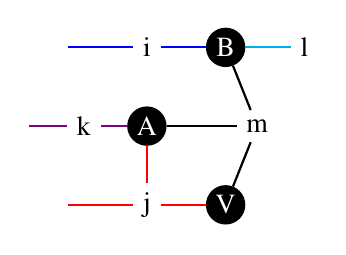
\begin{tikzpicture}[
    dot/.style = {circle, fill, minimum size=#1,
                inner sep=0pt, outer sep=0pt},
    dot/.default = 6pt  % size of the circle diameter 
                    ]  
    \def\dx{0};
    \def\r{0.5cm}
    \def\sr{0.15cm}
    \def\ax{0}
    \def\ay{0}
    \def\bx{1}
    \def\by{1}
    \def\cx{1}
    \def\cy{-1}
    \node[color=white,fill=black,dot=\r] at (\ax+\dx,\ax) (a) {A};
    \node[color=white,fill=black,dot=\r] at (\bx+\dx,\by) (b) {B};
    \node[color=white,fill=black,dot=\r] at (\cx+\dx,\cy) (v) {V};
    \node[color=transparent,draw=transparent,dot=0] at (\ax-1,\by) (o1) {};
    \node[color=transparent,draw=transparent,dot=0] at (\ax-1.5,\ay) (o2) {};
    \node[color=transparent,draw=transparent,dot=0] at (\ax-1,\cy) (o3) {};
    \node at (\ax-0.8,\ay) (k) {k};
    \node at (\bx+0.4,\ay) (m) {m};
    \node at (\ax,\cy) (j) {j};
    \node at (\bx+1,\by) (l) {l};
    \node at (\bx-1,\by) (i) {i};
    \draw[color=blue,thick] (i) -- (b);
    \draw[color=blue,thick] (i) -- (o1);
    \draw[color=cyan,thick] (l) -- (b);
    \draw[color=violet,thick] (k) -- (a);
    \draw[color=violet,thick] (k) -- (o2);
    \draw[color=black,thick] (b) -- (m);
    \draw[color=black,thick] (m) -- (a);
    \draw[color=black,thick] (m) -- (v);
    \draw[color=red,thick] (a) -- (j);
    \draw[color=red,thick] (v) -- (j);
    \draw[color=red,thick] (o3) -- (j);
\end{tikzpicture}}
\end{example}

\section{Generic programming tensor contractions}\label{sec:generic}
\purple{On a second read of this
section, I think that the clarity could be improved. My understanding is this is the flow:
We would like to use generic programming, where we write code that works regardless
of input type, and is optimized on all input types without sacrificing efficiency. In
general, we can write code such that a function runs correctly regardless of the input
data type. This is easy to do for dynamically typed languages like Python, which only
verify and enforce the rules for the input data type at run time (called type-checking).
However, when the input data type is only checked at run time (as opposed to when the
code is compiled), type-specific optimization cannot be used. High efficiency is only
achieved in statically typed languages, where modern compiling technology allows the
function to be individually optimized for each input data type (then give C++/Julia
examples).}\blue{how about now?}
In previous works relating tensor networks and combinatoric problems~\cite{Kourtis2019, Biamonte2017},
the elements in the tensor networks are limited to standard number types such as floating point numbers and integers.
%Owning to the development of modern compiling technology, we no longer need to restrict our imagination to standard number types.
In fact, the elements in a tensor does not have to be a regular number type,
 or even a field (since division is not used in tensor contraction).
One can use the same tensor contraction program for different purposes with different tensor element types,
and this idea of using the same program for different purposes is also called the generic programming in computer science:

\begin{definition}[Generic programming ~\cite{Stepanov2014}]
   Generic programming is an approach to programming that focuses on designing algorithms and data structures so that they work in the most general setting without loss of efficiency.
\end{definition}
This definition of generic programming covers two major aspects: ``work in the most general setting'' and ``with out loss of efficiency''.
By in the most general setting, we mean that a single program should work correctly for different input data types. For example, 
%\purple{I think the following paragraph could be clarified. When you read the definition of generic programming, it's not clear what ``in the most general setting'' means. My understanding is it just means that the program will work regardless of the input data type - it would be good to say this explicitly. }
%\blue{This definition is from the book I cited, I also do not like ``in the most general setting'', maybe we just use our version?}
%\purple{I also think the way it is written takes a while to understand what dynamically versus statically typed languages are. The definition, “When these languages “see” a new input type, the compiler can recompile the generic program for the new type.” comes rather late in the paragraph.}
%\xpurple{Also, while I know what you mean, concepts like “inlining immutable elements” and “cache miss rate” would be
%lost on someone only with a physics background.}
%This definition of generic programming contains two major aspects: a single program works in the most general setting and efficiency.
%To understand the first aspect on generality,
suppose we want to write a function that raises an element to a power, $f(x, n) := x^n$.
One can easily write a function for standard number types that computes the power of $x$ in $O \left( \log(n) \right)$ steps using the multiply and square trick.
Generic programming does not require $x$ to be a standard number type,
instead it treats $x$ as an element with an associative multiplication operation $\odot$ and a multiplicative identity $\mymathbb{1}$.
In such a way, when the program takes a matrix as an input, it computes the matrix power without extra efforts.
The second aspect is about the efficiency. For dynamically typed languages, such as Python,
one can easily write very general codes, but the efficiency is not guaranteed; for example, the speed of computing the matrix multiplication between two numpy arrays with python objects as elements is much slower than statically typed languages such as C++ and Julia~\cite{Bezanson2012}.
C++ uses templates for generic programming while Julia takes advantage of just-in-time compilation and multiple dispatch.
When these languages ``see'' a new input type, the compiler can recompile the generic program for the new type.
A myriad of optimizations can be done during the compilation, such as optimize the memory layout of immutable elements with fixed sizes in an array to speed up the array indexing.
In Julia, arrays with immutable elements with fixed sizes can even be compiled to GPU devices for faster computation~\cite{Besard2018}.

This motivates us to think about what is the most general tensor element type allowed in a tensor network contraction program.
We find that, as long as the algebra of tensor elements forms a commutative semiring, the tensor network contraction will be doable and the result will be independent of the contraction order.
Here, a commutative semiring is a field without additive inverse and multiplicative inverse.
Giving up these nice properties of a field means a lot to tensor computation: tensor network compression algorithms might be not applicable because matrix factorization is NP-hard for commutative semirings~\cite{Shitov2014}, and matrix multiplication faster than $O(n^3)$ does not exist for an algebra without additive inverse~\cite{Kerr1970}.
But here, we only use the commutative properties of an algebra for the purpose of tensor network contraction orders optimization.
To define a commutative semiring with the addition operation $\oplus$ and the multiplication operation $\odot$ on a set $S$, the following relations must hold for any arbitrary three elements $a, b, c \in S$.
\begin{align*}
(a \oplus b) \oplus c = a \oplus (b \oplus c) & \hspace{5em}\text{$\triangleright$ commutative monoid $\oplus$ with identity $\mymathbb{0}$}\\
a \oplus \mymathbb{0} = \mymathbb{0} \oplus a = a &\\
a \oplus b = b \oplus a &\\
&\\
(a \odot b) \odot c = a \odot (b \odot c)  &   \hspace{5em}\text{$\triangleright$ commutative monoid $\odot$ with identity $\mymathbb{1}$}\\
a \odot  \mymathbb{1} =  \mymathbb{1} \odot a = a &\\
a \odot b = b \odot a &\\
&\\
a \odot (b\oplus c) = a\odot b \oplus a\odot c  &  \hspace{5em}\text{$\triangleright$ left and right distributive}\\
(a\oplus b) \odot c = a\odot c \oplus b\odot c &\\
&\\
a \odot \mymathbb{0} = \mymathbb{0} \odot a = \mymathbb{0}
\end{align*}
%We require the algebra being multiplicative commutative because the contraction order optimizer will change the multiplication order of elements, while we require that the contraction order does not change the contraction results.
In the following sections, we show how to compute a number of properties of independent sets by designing tensor element types as specific commutative semirings without changing the tensor network contraction program~\cite{Stepanov2014}.
The Venn diagram in \Fig{fig:venn-diagram} shows the algebras we will introduce in the main text and their relation, and Table~\ref{tbl:generictypes} summarizes those properties that can be computed by various tensor element types.



\begin{figure}[th]
   \centering
\centerline{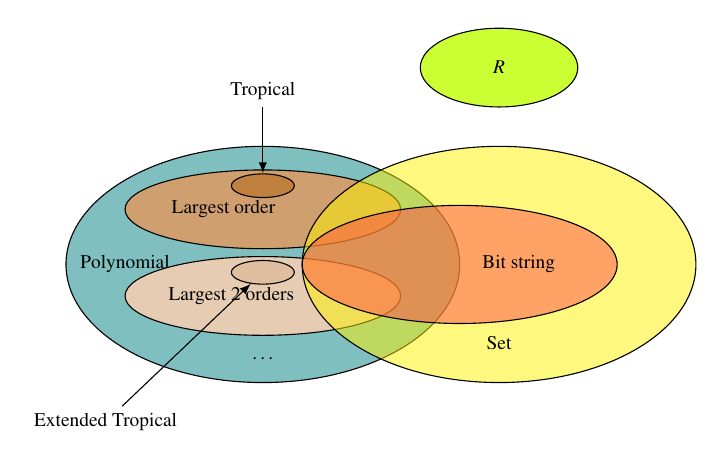
\begin{tikzpicture}[]
    \scriptsize
    \node[draw,fill=lime!80,fill opacity=1, text opacity=1.0,ellipse,minimum width=2cm, minimum height=1cm,inner sep=0pt] at (0, 2.5) (R) {$\mathbbm{R}$};
    \def\dx{-3};
    \node[draw,fill=teal!50,fill opacity=1, text opacity=1.0,ellipse,minimum width=5cm, minimum height=3cm,inner sep=0pt] at (\dx, 0) (PN) {\hspace{-3.5cm}Polynomial};
    \node[draw,fill=brown!75,fill opacity=1, text opacity=1.0,ellipse,minimum width=3.5cm, minimum height=1.0cm,inner sep=0pt] at (\dx, 0.7) (P1) {\hspace{-1.0cm}Largest order};
    \node[draw,fill=brown!40,fill opacity=1, text opacity=1.0,ellipse,minimum width=3.5cm, minimum height=1.0cm,inner sep=0pt] at (\dx, -0.4) (P2) {\hspace{-0.8cm}Largest 2 orders};
    \node[draw,fill=brown,fill opacity=1, text opacity=1.0,ellipse,minimum width=0.8cm, minimum height=0.3cm,inner sep=0pt] at (\dx, 1.0) (T) {};
    \node[draw,fill=brown!50,fill opacity=1, text opacity=1.0,ellipse,minimum width=0.8cm, minimum height=0.3cm,inner sep=0pt] at (\dx, -0.1) (T2) {};
    \node at (\dx, -1.2) {$\ldots$};
    \node[above = 1cm] at (T) (textT) {Tropical};
    \node[below = 2cm, left=4cm] (textT2) {Extended Tropical};
    \draw[black,-latex] (textT) -- (T);
    \draw[black,-latex] (textT2) -- (T2);

    % set and set sampler
    \node[draw,fill=yellow,fill opacity=0.5, text opacity=1.0,ellipse,minimum width=5cm, minimum height=3cm,inner sep=0pt] at (0, 0) (SN) {};
    \node[below of=1] at (SN) {Set};
    \node[draw,fill=red!70,fill opacity=0.5, text opacity=1.0,ellipse,minimum width=4cm, minimum height=1.5cm,inner sep=0pt] at (-0.5, 0) (S1) {\hspace{1.5cm}Bit string};
\end{tikzpicture}}

    \caption{The the tensor network element types used in this work, while the purpose of these element types can be found in \Tbl{tbl:generictypes}.
    The overlap between two algebra indicates that a new algebra can be created by combining those two types of algebra. ``Largest order'' and ``Largest 2 orders'' mean truncating the polynomial by only keeping its largest or largest two orders.}
     \label{fig:venn-diagram}
\end{figure}

\begin{table}[t!]\centering
\begin{minipage}{\columnwidth}
\ra{1.3}
        \begin{tabularx}{\textwidth}{sb}\toprule
            \hline
   \textbf{Element type}     & \textbf{Solution space property} \\
   {$\mathbbm{R}$}     & {Counting of all independent sets} \\
   {Polynomial} (\Eq{eq:polynomial})     & {Independence polynomial} \\
   {Tropical (\Eq{eq:tropical})}    & {Maximum independent set size} \\
   {Extended tropical of order $k$ (\Eq{eq:ext-tropical})}    & {Largest $k$ independent set sizes} \\
   {Polynomial truncated to $k$-th order (\Eq{eq:countingtropical} and \Eq{eq:max2poly})}     & {$k$ largest independent sizes and their degeneracy} \\
   {Set} (\Eq{eq:set})     & {Enumeration of independent sets} \\
   {Sum-Product expression tree} (\Eq{eq:expr})     & {Sampling of independent sets} \\
   {Polynomial truncated to largest order combined with bit string} (\Eq{eq:singleconfig})     & {Maximum independent set size and one of such configurations} \\
   {Polynomial truncated to $k$-th order combined with set} (\Eq{eq:countingtropicalset})    & {$k$ largest independent set sizes and their enumeration} \\
            \bottomrule
        \end{tabularx}
    \caption{Tensor element types and the independent set properties that can be computed using them.}\label{tbl:generictypes}
\end{minipage}
\end{table}

\section{Tensor network representation of independent sets} \label{sec:tnmap}
This section is about reducing the independent set problem to a tensor network contraction problem.
For people with physics background, we suggest using an alternative approach described in \App{sec:energymodel} to understand this reduction from an energy model.
Let $G=(V,E)$ be a weighted undirected graph with each vertex $v\in V$ being associated with a weight $w_v$.
An independent set $I \subseteq V$ is a set of vertices that for any vertex pair $u,v \in I$, $(u, v) \not\in E$,
and we denote the maximum independent set (MIS) size $\alpha(G) \equiv \max_{I}\sum_{v\in I}w_v$. 
We map a vertex $v\in V$ to a label $s_v \in \{0, 1\}$ of dimension $2$ in a tensor network, where we use $0$ ($1$) to denote a vertex is absent (present) in the set.
For each label $s_v$, we defined a parametrized rank-one vertex tensor $W(x_v, w_v)$ as
\begin{equation}
    W(x_v, w_v) = \left(\begin{matrix}
        1_v \\
        x_v^{w_v}
    \end{matrix}\right).\label{eq:vertextensor}
\end{equation}
where subscripts are used to annotate different vertices in configuration enumeration and sampling.
One can index tensor elements by subscripting tensors, e.g.\ $W(x_v, w_v)_0=1_v$ is the first element associated with $s_v=0$ and $W(x_v, w_v)_1=x_v^{w_v}$ is the second element associated with $s_v=1$.
Similarly, on each edge $(u, v)$, we define a matrix $B$ indexed by $s_u$ and $s_v$ as
\begin{equation}
    \qquad \quad 
       B = \left(\begin{matrix}
        1  & 1\\
        1 & 0
    \end{matrix}\right). \label{eq:edgetensor}
\end{equation}
The corresponding tensor network contraction gives
\begin{equation}\label{eq:idp}
    P(G, \{x_1^{w_1}, x_{2}^{w_2}, \ldots,x_{|V|}^{w_{|V|}}\}) = \sum\limits_{s_1, s_2, \ldots, s_{|V|} = 0}^{1} \prod\limits_{v\in V} W(x_v, w_v)_{s_v} \prod\limits_{(w,v) \in E} B_{s_w s_v},
\end{equation}
where the summation runs over all vertex configurations $\{s_1, s_{2}, \ldots,s_{|V|}\}$ and accumulates the product of tensor elements to the output $P$.
The edge tensor element $B_{s_{i}=1, s_{j}=1} = 0$ encodes the independent set constraint, meaning vertex $i$ and $j$ cannot be both in the independent set if they are connected by an edge $(i,j)$.

\begin{example}\label{eg:twonode}
In the following, we show a minimum example of mapping the independent problem of a 2 vertex complete graph K2 (left) to a tensor network (right).

\centerline{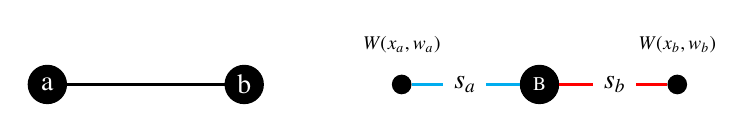
\begin{tikzpicture}[
dot/.style = {circle, fill, minimum size=#1,
            inner sep=0pt, outer sep=0pt},
dot/.default = 6pt  % size of the circle diameter 
                ]  
    \def\dx{0};
    \def\r{0.5cm}
    \def\wr{0.25cm}
    \node[dot=\r, fill=black] at (\dx,0) (a) {\color{white}{a}};
    \node[dot=\r, fill=black] at (2.5+\dx,0) (b) {\color{white}{b}};
    \draw [black,thick] (a) -- (b);

    \def\dx{5};
    \def\r{0.25cm}
    \foreach \x/\y/\e in {1.25/0/ab}
        \node[color=black,fill=black,dot=2*\r] at (\x+\dx,\y) (\e) {\scriptsize \color{white}{B}};
    \foreach \x/\y/\v in {0.3/0/a, 2.2/0/b}
        \node[color=black] at (\x+\dx,\y) (s\v) {$s_\v$};
    \foreach \x/\y/\v in {-0.5/0/a, 3.0/0.0/b}{
        \node[dot=\wr, color=black] at (\x+\dx,\y) (w\v) {};
        \node at (\x+\dx,\y+0.5) () {\scriptsize \color{black}{$W(x_\v, w_\v)$}};
    }
    \draw [cyan,thick] (wa) -- (sa);
    \draw [cyan,thick] (sa) -- (ab);
    \draw [red,thick] (wb) -- (sb);
    \draw [red,thick] (sb) -- (ab);
\end{tikzpicture}}

In the graphical representation of tensor network on the right panel,
we use a circle to represent a tensor, a hyperedge in cyan color to represent the degree of freedom $s_a$,
and a hyperedge in red color to represent a degree of freedom $s_b$.
Tensors sharing a same degree of freedom are connected by that hyperedge.
The contraction of this tensor network can be evaluated manually:
\begin{equation}
    \begin{split}
    P({\rm K2},\{x_a^{w_a}, x_b^{w_b}\}) &=
    \left(\begin{matrix} 1 & x_a^{w_a} \end{matrix}\right)
    \left(\begin{matrix} 1 & 1\\ 1  & 0 \end{matrix}\right)
    \left(\begin{matrix} 1 \\ x_b^{w_b} \end{matrix}\right)\\
    &= 1 + x_a^{w_a} + x_b^{w_b}
    \end{split}
\end{equation}
The resulting polynomial represents 3 different independent sets $\{\}$, $\{a\}$ and $\{b\}$, with weights being $0$, $w_a$ and $w_b$ respectively.
\end{example}
 
In general, it is not computationally efficient to evaluate \Eq{eq:idp} by directly summing up the $2^{|V|}$ products. %, which scales exponentially as the number of vertices.
%\purple{Perhaps explicitly say what this scales as?}\blue{I am not sure explicitly saying ``scales exponentially as the number of vertices'' is helpful, because treewidth often scales linearly as number of vertices, so tensor network also scales exponentially as the number vertices in most cases.}
The standard approach to evaluate a random tensor network is: first find a good pair-wise tensor contraction order as a binary tree, and then contract two tensors a time by this order.
An optimal tensor network contraction order corresponds to an optimal tree decomposition of its line graph and the largest intermediate tensor has a rank equal to the tree width of this optimal tree decomposition~\cite{Markov2008}.
In practice, it is difficult to find an optimal contraction order for large tensor networks because finding the treewidth itself is NP-hard.
However, it is easy to find a close to optimal contraction order in typically a few minutes with a heuristic contraction order finding algorithm~\cite{Kourtis2019,Kalachev2021} utilizing the associativity and commutativity of tensor contraction.
%The pairwise tensor contraction also makes it possible to utilize basic linear algebra subprograms (BLAS) functions to speed up the computation for certain tensor element types.
For large scale applications, it is also possible to slice over certain degrees of freedom to reduce the space complexity, i.e.
loop and accumulate over certain degrees of freedom so that one can have a smaller tensor network inside the loop due to the removal of these degrees of freedom, which might have a smaller space complexity.

\begin{example}\label{eg:tensorcontraction}
In the following, we map a 5-vertex graph (left) to a tensor network (right) and show how the contraction order reduces the time and space complexities.
    
\centerline{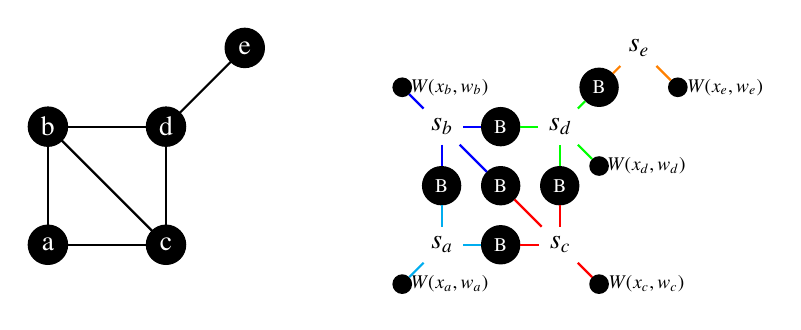
\begin{tikzpicture}[
dot/.style = {circle, fill, minimum size=#1,
            inner sep=0pt, outer sep=0pt},
dot/.default = 6pt  % size of the circle diameter 
                ]  
    \def\dx{0};
    \def\r{0.25cm}
    \filldraw[fill=black] (\dx,0) circle [radius=\r];
    \filldraw[fill=black] (\dx,1.5) circle [radius=\r];
    \filldraw[fill=black] (1.5+\dx,0) circle [radius=\r];
    \filldraw[fill=black] (1.5+\dx,1.5) circle [radius=\r];
    \filldraw[fill=black] (2.5+\dx,2.5) circle [radius=\r];
    \draw [black,thick] (\dx,0) -- (\dx,1.5);
    \draw [black,thick] (\dx,0) -- (1.5+\dx,0);
    \draw [black,thick] (\dx,1.5) -- (1.5+\dx,1.5);
    \draw [black,thick] (1.5+\dx,0) -- (1.5+\dx,1.5);
    \draw [black,thick] (1.5+\dx,0) -- (\dx,1.5);
    \draw [black,thick] (2.5+\dx,2.5) -- (1.5+\dx,1.5);
    \node[color=white] at (\dx,0) {a};
    \node[color=white] at (\dx,1.5) {b};
    \node[color=white] at (1.5+\dx,0) {c};
    \node[color=white] at (1.5+\dx,1.5) {d};
    \node[color=white] at (2.5+\dx,2.5) {e};
    \def\dx{5};
    \def\r{0.25cm}
    \foreach \x/\y/\e in {0.75/0/ac, 0/0.75/ab, 1.5/0.75/cd, 0.75/1.5/bd, 0.75/0.75/bc, 2/2/de}
        \node[color=white,fill=black,dot=2*\r] at (\x+\dx,\y) (\e) {\scriptsize B};
    \foreach \x/\y/\v in {0/0/a, 0/1.5/b, 1.5/0/c, 1.5/1.5/d, 2.5/2.5/e}
        \node[color=black] at (\x+\dx,\y) (\v) {$s_\v$};
    \foreach \x/\y/\v in {-0.5/-0.5/a, -0.5/2.0/b, 2.0/-0.5/c, 2.0/1.0/d, 3.0/2.0/e}
        \node[color=white,fill=black,dot=\r] at (\x+\dx,\y) (\v\v) {};
    \foreach \x/\y/\v in {-0.5/-0.5/a, -0.5/2.0/b, 2.0/-0.5/c, 2.0/1.0/d, 3.0/2.0/e}
        \node[color=black] at (\x+\dx+0.6,\y) {\scriptsize $W(x_\v, w_\v)$};
    \draw [cyan,thick] (a) -- (aa);
    \draw [cyan,thick] (a) -- (ab);
    \draw [cyan,thick] (a) -- (ac);
    \draw [blue,thick] (b) -- (bb);
    \draw [blue,thick] (b) -- (ab);
    \draw [blue,thick] (b) -- (bc);
    \draw [blue,thick] (b) -- (bd);
    \draw [red,thick] (c) -- (cc);
    \draw [red,thick] (c) -- (ac);
    \draw [red,thick] (c) -- (bc);
    \draw [red,thick] (c) -- (cd);
    \draw [green,thick] (d) -- (dd);
    \draw [green,thick] (d) -- (bd);
    \draw [green,thick] (d) -- (de);
    \draw [green,thick] (d) -- (cd);
    \draw [orange,thick] (e) -- (ee);
    \draw [orange,thick] (e) -- (de);
\end{tikzpicture}}

One can represent a possible pair-wise contraction of tensors as a binary tree structure:

\centerline{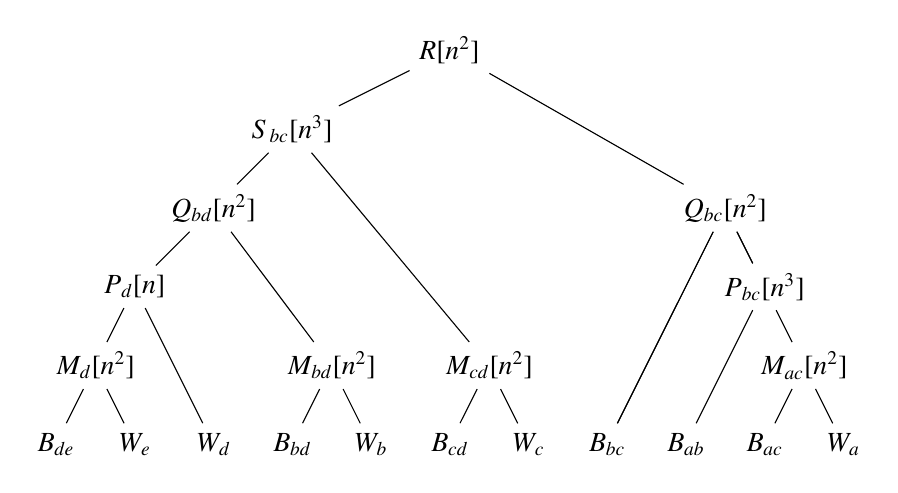
\begin{tikzpicture}[]
    \def\dx{0};
    \def\dy{0};
    \def\d{1};
    \def\a{1.0};
    \def\b{1};
    \def\ya{-1.0};
    \def\yb{-0.8};
    \node[] at (\dx+5*\a, \dy+5*\b) (R1) {$R[n^2]$};
    \node[] at (\dx+3*\a, \dy+4*\b) (S1) {$S_{bc}[n^3]$};
    \node[] at (\dx+2*\a, \dy+3*\b) (Q1) {$Q_{bd}[n^2]$};
    \node[] at (\dx+8.5*\a, \dy+3*\b) (Q2) {$Q_{bc}[n^2]$};
    \node[] at (\dx+\a, \dy+2*\b) (P1) {$P_{d}[n]$};
    \node[] at (\dx+9*\a, \dy+2*\b) (P2) {$P_{bc}[n^3]$};
    \node[] at (\dx+0.5*\d, \dy+\b) (M1) {$M_{d}[n^2]$};
    \node[] at (\dx+3.5*\d, \dy+\b) (M2) {$M_{bd}[n^2]$};
    \node[] at (\dx+5.5*\d, \dy+\b) (M3) {$M_{cd}[n^2]$};
    \node[] at (\dx+9.5*\d, \dy+\b) (M4) {$M_{ac}[n^2]$};
    \node[] at (\dx, \dy) (Bde) {$B_{de}$};
    \node[] at (\dx+\d, \dy) (We) {$W_e$};
    \node[] at (\dx+2*\d, \dy) (Wd) {$W_d$};
    \node[] at (\dx+3*\d, \dy) (Bbd) {$B_{bd}$};
    \node[] at (\dx+4*\d, \dy) (Wb) {$W_b$};
    \node[] at (\dx+5*\d, \dy) (Bcd) {$B_{cd}$};
    \node[] at (\dx+6*\d, \dy) (Wc) {$W_c$};
    \node[] at (\dx+7*\d, \dy) (Bbc) {$B_{bc}$};
    \node[] at (\dx+8*\d, \dy) (Bab) {$B_{ab}$};
    \node[] at (\dx+9*\d, \dy) (Bac) {$B_{ac}$};
    \node[] at (\dx+10*\d, \dy) (Wa) {$W_a$};
    \draw[] (Bde) -- (M1);
    \draw[] (We) -- (M1);
    \draw[] (Bbd) -- (M2);
    \draw[] (Wb) -- (M2);
    \draw[] (Bcd) -- (M3);
    \draw[] (Wc) -- (M3);
    \draw[] (Bac) -- (M4);
    \draw[] (Wa) -- (M4);
    \draw[] (M1) -- (P1);
    \draw[] (Wd) -- (P1);
    \draw[] (Bab) -- (P2);
    \draw[] (M4) -- (P2);
    \draw[] (P1) -- (Q1);
    \draw[] (M2) -- (Q1);
    \draw[] (Bbc) -- (Q2);
    \draw[] (P2) -- (Q2);
    \draw[] (Bbc) -- (Q2);
    \draw[] (P2) -- (Q2);
    \draw[] (Q1) -- (S1);
    \draw[] (M3) -- (S1);
    \draw[] (S1) -- (R1);
    \draw[] (Q2) -- (R1);
\end{tikzpicture}}
% \small{
% \begin{align*}
%     &\sum_{s_a,s_b,s_c,s_d,s_e} W(x_a, w_a)_{s_a} W(x_b, w_b)_{s_b} W(x_c, w_c)_{s_c} W(x_d, w_d)_{s_d} W(x_e, w_e)_{s_e} B_{s_a s_b} B_{s_b s_d} B_{s_c s_d} B_{s_a s_c} B_{s_b s_c} B_{s_d s_e}\\
%     =&\sum_{s_b,s_c}\left(\sum_{s_d}\left(\left(\left(\left(\sum_{s_e}B_{s_d s_e}W(x_e,w_e)_{s_e}\right) W(x_d,w_d)_{s_d}\right) \left(B_{s_bs_d} W(x_b, w_b)_{s_b}\right)\right) \left(B_{s_cs_d} W(x_c, w_c)_{s_c}\right)\right)\right.\\
%     &\phantom{XXX}\left.\left(B_{s_bs_c}\left(\sum_{s_a}B_{s_as_b}\left(B_{s_as_c}W(x_a,w_a)_{s_a}\right)\right)\right)\right)\\
%     =&1 + x_a^{w_a} + x_b^{w_b} + x_c^{w_c} + x_d^{w_d} + x_e^{w_e} + x_a^{w_a}x_d^{w_d} + x_a^{w_a}x_e^{w_e} + x_c^{w_c}x_e^{w_e} + x_b^{w_b}x_e^{w_e}
%     %=&1+5x+4x^2 \qquad \quad (x_{i} = x, w_{i}=1).
% \end{align*}}
The contraction process goes from bottom to top, where the root stores the contraction result that we want, the leaves are tensors in our tensor network while the rest nodes are all intermediate contraction results.
Tensor subscripts are indices so that the number of subscripts indicates the space complexity to store this tensor. The contraction complexity to generate a tensor is annotated in the square brackets, where $n$ is the dimension of degrees of freedom, which in our case is $2$.
One can easily check the largest tensor during computing has space complexity $O(n^2)$ and this is optimal, i.e. the treewidth of the original $5$-vertex graph is $2$, and the time complexity is $O(n^3)$, which is much smaller than that of direct enumeration $O(n^5)$.
\end{example}

\section{Independence polynomial}\label{sec:indpoly}
Let $x_i = x$ and $w_i = 1$, the evaluation of \Eq{eq:idp} corresponds to the independence polynomial~\cite{Harvey2018,Ferrin2014}.
which is a useful graph characteristic related to, for example, the partition functions~\cite{Lee1952,Yang1952} and Euler characteristics of the independence complex~\cite{Bousquet2008, Levit2009}.
The independence polynomial is an important graph polynomial that contains the counting information of independent sets. It is defined as
\begin{equation}\label{eq:idpdef}
I(G, x) = \sum_{k=0}^{\alpha(G)} a_k x^k,
\end{equation}
where $a_k$ is the number of independent sets of size $k$ in graph $G=(V,E)$. The total number of independent sets is thus equal to $I(G, 1)$.
Its connection to \Eq{eq:idp} can be understood as follows: the product over vertex tensor elements produces a factor $x^k$, where $k=\sum_i s_i$ counts the set size,
and the product over edge tensor elements gives a factor $1$ for a configuration being in an independent set and $0$ otherwise. The summation counts the number of independent sets of size $k$. 
By assigning a real number to $x$, one can evaluate this independence polynomial for this specific value directly by contracting this tensor network.
However, instead of evaluating this polynomial for a certain value, we are more interested in knowing the coefficients of this polynomial, because this quantity tells us the counting of independent sets at each size.
To achieve this, let us first elevate the tensor elements $0$s and $1$s in tensors $W(x, 1)$ and $B$ from integers and floating point numbers to the additive identity,
$\mymathbb{0}$, and multiplicative identity, $\mymathbb{1}$, of a commutative semiring as discussed in Sec.~\ref{sec:generic}.
\purple{I'd
say that you're about to describe this semiring, otherwise it seems like you're going to
use the general definition of the semiring rather than a specific type of semiring}\blue{from $1$ to $\mymathbb{1}$ and $0$ to $\mymathbb{0}$ applies for a general semiring, I haven't change this part, let's discuss to make sure I understand your point.}
Let us create a polynomial type and represent a polynomial $a_0 + a_1 x + \ldots + a_k x^k$ as a coefficient vector $a = (a_0, a_1, \ldots, a_k) \in \mathbb{R}^k$, so, e.g., $x$ is represented as $(0, 1)$.
We define the algebra between the polynomials $a$ of order $k_a$ and $b$ of order $k_b$ as
\begin{equation}
    \eqname{PN}
    \begin{split}
    a \oplus b &= (a_0 + b_0, a_1 + b_1, \ldots, a_{\max(k_a, k_b)} + b_{\max(k_a, k_b)}),\\
    a \odot b &= (a_0 + b_0, a_1b_0 + a_0b_1, a_{2}b_{0} + a_{1}b_{1} + a_{0}b_{2},  \ldots, a_{k_a} b_{k_b}),\\
    \mymathbb{0} &= (),  \\
    \mymathbb{1} &= (1).\label{eq:polynomial}
    \end{split}
\end{equation}
Here, the multiplication operation can be evaluated in time $O(k\log(k))$, where $k=\max{k_a, k_b}$, using the convolution theorem~\cite{Schonhage1971}.
These operations are standard addition and multiplication operations of polynomials, and the polynomial type forms a commutative ring. The tensors $W$ and $B$ can thus be written as 
\begin{equation}
    W^{\rm PN} = \left(\begin{matrix}
        \mymathbb{1} \\
        (0,1)
    \end{matrix}\right),   
    \qquad \qquad
        B^{\rm PN} = \left(\begin{matrix}
        \mymathbb{1}  & \mymathbb{1} \\
        \mymathbb{1} & \mymathbb{0}
    \end{matrix}\right).
\end{equation}
By contracting the tensor network with the polynomial type, we have the exact representation of the independence polynomial.
In practise, using the polynomial type suffers a space overhead proportional to $\alpha(G)$ because each polynomial requires a vector of such size to store the coefficients. 
One may argue that one can first evaluate this polynomial at different $x$ being a real number,
and then apply the Gaussian elimination to fit the coefficients of this polynomial.
This seemingly more time and space efficient approach suffers from severe issues in practise.
The data ranges of standard integer types are too small to cover many practical using cases,
while the floating point numbers may have round off error that much larger than the value itself
due to the fact that the number of sets at different sizes may vary tens or even hundreds of orders and this makes the small coefficients can not be retrieved correctly by fitting.
For the purpose of evaluating these coefficients, we refer readers to \App{sec:finitefield}, where we provide an accurate and memory efficient method to find the polynomial by fitting it in a finite field.
Alternatively, one can use the method in \App{sec:fft} to fit this polynomial more time efficiently with complex numbers with controllable round off errors.
For the purpose of discussion in the main text, let us stick to this less efficient polynomial algebra.

\section{Maximum independent sets and its counting}\label{sec:counting}
\subsection{Tropical algebra for finding the MIS size and counting MISs}
The MIS size $\alpha(G)$, or the independence number is an important graph characteristics.
The method we use to compute this quantity is based on the following observations.
Let $x=\infty$, the independence polynomial in the previous section becomes
\begin{equation}
I(G, \infty) = \lim_{x\rightarrow \infty}\sum_{k=0}^{\alpha(G)}a_k x^k = a_{\alpha(G)} \infty^{\alpha(G)},
\end{equation}
where all terms except the largest order vanish. We can thus replace the polynomial type $a = (a_0, a_1, \ldots, a_k)$ with a new type that has two fields: the largest exponent $k$ and its coefficient $a_k$.
From this, we can define a new algebra as
\begin{equation}
    \eqname{P1}
\begin{split}
    a_x\infty^x \oplus a_y\infty^y &= \begin{cases}
        (a_x + a_y)\infty^{\max(x,y)}, & x = y\\
        a_y\infty^{\max(x,y)}, & x < y\\
        a_x\infty^{\max(x,y)}, & x > y
    \end{cases}, \\
    a_x\infty^x \odot a_y\infty^y &= a_x a_y\infty^{x+y}\\
    \mymathbb{0} &= 0\infty^{-\infty}\\
    \mymathbb{1} &= 1\infty^{0}.
\end{split}%& \text{\rlap{(P1)}}
\label{eq:countingtropical}
\end{equation}
Note here, in order to define the zero element, we have generalized the previous polynomial to the Laurent polynomial.
To implement this algebra programmatically, we create a data type with two fields $(x, a_x)$ to store the MIS size and its counting,
and define the above operations and constants correspondingly.
If one is only interested in finding the MIS size, one can drop the counting field.
The algebra of the exponents becomes the max-plus tropical algebra~\cite{Maclagan2015, Moore2011}:
\begin{equation}\eqname{T}
    \begin{split}
        x \oplus y &= \max(x,y)\\
        x \odot y &= x + y\\
        \mymathbb{0} &= -\infty\\
        \mymathbb{1} &= 0.
    \end{split}\label{eq:tropical}
\end{equation}
Algebra \Eq{eq:tropical} and \Eq{eq:countingtropical} are the same as those used in Liu et al.~\cite{Liu2021} to calculate and count spin glass ground states.
For independent set calculations here, the vertex tensor and edge tensor becomes:
\begin{equation}
    W^{\rm T} = \left(\begin{matrix}
        \mymathbb{1} \\
        \infty
    \end{matrix}\right),   
    \qquad \qquad
        B^{\rm T} = \left(\begin{matrix}
        \mymathbb{1}  & \mymathbb{1} \\
        \mymathbb{1} & \mymathbb{0}
    \end{matrix}\right).
\end{equation}

\subsection{Truncated polynomial algebra for counting independent sets of large size}
Instead of counting just the MISs, one may also be interested in counting the independent sets with largest several sizes.
For example, if one is interested in counting only $a_{\alpha(G)}$ and $a_{\alpha(G)-1}$, we can define a truncated polynomial algebra by keeping only the largest two coefficients in the polynomial in \Eq{eq:polynomial} as:
\begin{equation}
    \eqname{P2}
    \begin{split}
    a \oplus b &= (a_{\max(k_a, k_b)-1} + b_{\max(k_a, k_b)-1}, a_{\max(k_a, k_b)} + b_{\max(k_a, k_b)}),\\
    a \odot b &= (a_{k_a-1} b_{k_b}+a_{k_a} b_{k_b-1}, a_{k_a} b_{k_b}),\\
    \mymathbb{0} &= (), \\
    \mymathbb{1} &= (1).\label{eq:max2poly}
    \end{split}
\end{equation}
In the program, we thus need a data structure that contains three fields, the largest order $k$, and the coefficients for the two largest orders $a_k$ and $a_{k-1}$.
This approach can clearly be extended to calculate more independence polynomial coefficients and is more efficient than calculating the entire independence polynomial.
Similarly, one can also truncate the polynomial and keep only its smallest several orders,
which can be used for e.g. counting the maximal independent sets with smallest cardinality,
where a maximal independent set is an independent set that can not be made larger by adding a new vertex into the it without violating the independence constraint.
As will be shown below, this algebra can also be extended to enumerate those large-size independent sets.

\section{Enumerating and sampling independent sets}\label{sec:enumeration}

\subsection{Set algebra for configuration enumeration}
The configuration enumeration of independent sets includes,
for example, the enumeration of all independent sets, the enumeration of all MISs and the enumeration of independent sets with maximum several sizes.
Recall that in the definition of a vertex tensor in \Eq{eq:vertextensor}, variables can carry labels, so that in the output polynomials, one can read out all independent sets directly.
The multiplication between labelled variables are commutative while the summation of labelled variables forms a set.
Intuitively, one can use a bit string as the representation of a labelled variable and use bit-wise or $\lor^\circ$ as the multiplication operation,
e.g. in a 5-vertex graph, $x_2$ can be represented as $01000$, $x_5$ can be represented as $00001$ and their multiplication $x_2x_5$ can be represented as $01000 \lor^\circ 00001 = 01001$.
To enumerate all independent sets, we designed an algebra defined on sets of bit strings:
\begin{equation}
\eqname{SN}
\begin{split}
    s \oplus t &= s \cup t\\
    s \odot t &= \{\sigma \lor^\circ \tau \, | \, \sigma \in s, \tau \in t\}\\
    \mymathbb{0} &= \{\}\\
    \mymathbb{1} &= \{0^{\otimes |V|}\}.
\end{split}\label{eq:set}
\end{equation}
where $s$ and $t$ are each a set of $|V|$-bit strings.
\begin{example}\label{eg:setalgebra}
    For elements being bit strings of length $5$, we have the following set algebra
\begin{equation*}
\begin{split}
    &\{00001\} \oplus \{01110, 01000\} = \{01110, 01000\} \oplus \{00001\} = \{00001,01110, 01000\}\\
    &\{00001\} \oplus \{\} = \{00001\}\\
&\\
    &\{00001\} \odot \{01110, 01000\} = \{01110, 01000\} \odot \{00001\} = \{01111, 01001\}\\
    &\{00001\} \odot \{\} = \{\}\\
    &\{00001\} \odot \{00000\} = \{00001\}.
\end{split}
\end{equation*}
\end{example}

To enumerate all independent sets, 
we initialize variable $x_{i}$ in the vertex tensor to $x_i = \{\boldsymbol{e}_{i}\}$, where $\boldsymbol{e}_i$ is a basis bit string of size $|V|$ that has only one non-zero value at location $i$.
The vertex and edge tensors are thus
\begin{equation}
    W^{\rm SN}(\{\boldsymbol{e}_{i}\}) = \left(\begin{matrix}
        \mymathbb{1} \\
        \{\boldsymbol{e}_{i}\}
    \end{matrix}\right),   
    \qquad \qquad
        B^{\rm SN} = \left(\begin{matrix}
        \mymathbb{1}  & \mymathbb{1} \\
        \mymathbb{1} & \mymathbb{0}
    \end{matrix}\right).
\end{equation}

This set algebra can serve as the coefficients in \Eq{eq:polynomial} to enumerate independent sets of all different sizes, \Eq{eq:countingtropical} to enumerate all MISs,
or \Eq{eq:max2poly} to enumerate all independent sets of size $\alpha(G)$ and $\alpha(G)-1$.
As long as the coefficients in a truncated polynomial forms a commutative semiring, the polynomial itself is still a commutative semiring.
For example, to enumerate only the MISs, with the tropical algebra, we can define $s_{k}\infty^k$,
where the coefficients follow the algebra in \Eq{eq:set} and the orders (exponents) follow the max-plus tropical algebra.
The combined operations become: 
\begin{equation}
\eqname{P1+SN}
\begin{split}
    s_x\infty^x \oplus s_y\infty^y &= \begin{cases}
        (s_x \cup s_y)\infty^{\max(x,y)}, & x = y\\
        s_y\infty^{\max(x,y)}, & x < y\\
        s_x\infty^{\max(x,y)}, & x > y
    \end{cases},\\
    s_x\infty^x \odot s_y\infty^y &= \{\sigma \lor^\circ \tau | \sigma \in s_x, \tau \in s_y\}\infty^{x+y},\\
    \mymathbb{0} &= \{\}\infty^{-\infty},\\
    \mymathbb{1} &= \{0^{\otimes |V|}\}\infty^{0}. \label{eq:countingtropicalset}
\end{split}
\end{equation}
Clearly, the vertex tensor and edge tensor become
\begin{equation}
    W^{\rm P1+SN}(\{\boldsymbol{e}_{i}\infty^1\}) = \left(\begin{matrix}
        \mymathbb{1} \\
        \{\boldsymbol{e}_{i}\}\infty^1
    \end{matrix}\right),   
    \qquad \qquad
        B^{\rm P1+SN} = \left(\begin{matrix}
        \mymathbb{1}  & \mymathbb{1} \\
        \mymathbb{1} & \mymathbb{0}
    \end{matrix}\right).
\end{equation}
The contraction of the corresponding tensor network yields an enumeration of all MIS configurations.
Direct implementing this algebra for configuration MISs might incur significant space overheads for keeping too many intermediate states not contributing to the final maximum independent sets,
one can avoid this issue by using the bounding technique in \App{sec:bounding}.
One may also be interested in a more studied enumeration of maximal independent sets~\cite{Bron1973, Eppstein2010, Johnson1988}. It will be discussed in \App{sec:maximal} since it requires using a different tensor network structure for the maximal independent set problem.

If one is interested in obtaining only a single MIS configuration, one can just keep a single configuration in the intermediate computations to save the computational effort.
Here is a new algebra defined on the bit strings, replacing the sets of bit strings in \Eq{eq:set}, 

\begin{equation}
\eqname{S1}
\begin{split}
    \sigma \oplus \tau &= \texttt{select}(\sigma, \tau), \\
    \sigma \odot \tau &= (\sigma\lor^\circ \tau),\\
    \mymathbb{0} &= 1^{\otimes |V|}, \\
    \mymathbb{1} &= 0^{\otimes |V|},
\end{split}\label{eq:singleconfig}
\end{equation}
where the \texttt{select} function picks one of $\sigma$ and $\tau$ by some criteria to make the algebra commutative and associative, e.g. by picking the one with a smaller integer value. In practise, it is completely fine to pick a random one (not commutative anymore) to generate a random MIS.

\subsection{Sampling extremely large configuration space}
When the graph size goes large, a set of configurations might be impossible to fit into any type of storage.
To get something meaningful out of configuration space, we use a binary sum-product expression tree as a compact representation of a set of configurations, i.e. instead of directly computing a set using the algebra in \Eq{eq:set}, we store the process of computing it.
A node in this tree is a quadruple $(type, data, left, right)$, where $type$ is one of
\texttt{LEAF}, \texttt{ZERO}, \texttt{SUM} and \texttt{PROD}, $data$ is a bit string as the content in a \texttt{LEAF} node,
$left$ and $right$ are left and right operands of a \texttt{SUM} or \texttt{PROD} node.

\begin{equation}
\eqname{EXPR}
\begin{split}
    s \oplus t &= (\texttt{SUM}, /, s, t)\\
    s \odot t &= (\texttt{PROD}, /, s, t)\\
    \mymathbb{0} &= (\texttt{ZERO}, /, /, /)\\
    \mymathbb{1} &= (\texttt{LEAF}, 0^{\otimes |V|}, /, /).
\end{split}\label{eq:expr}
\end{equation}
The vertex tensor and edge tensor become
\begin{equation}
    W^{\rm EXPR}((\texttt{LEAF},\boldsymbol{e}_i,/,/)) = \left(\begin{matrix}
        \mymathbb{1} \\
        (\texttt{LEAF},\boldsymbol{e}_i,/,/)
    \end{matrix}\right),   
    \qquad
        B^{\rm EXPR} = \left(\begin{matrix}
        \mymathbb{1}  & \mymathbb{1} \\
        \mymathbb{1} & \mymathbb{0}
    \end{matrix}\right).
\end{equation}

This algebra is a commutative semiring because we define the equivalence of two sum-product expression trees by comparing their expanded (using \Eq{eq:set}) forms, rather than their storages.
Except using the sum-product expression tree directly as tensor elements, one can also let it be the coefficients of a (truncated) polynomial so that one can have such trees for independent sets with largest several sizes.
Although one probably can not enumerate all configurations represented by a sum-product expression tree due to its extremely large size,
he can draw unbiased samples from it efficiently.
One starts from the root node, and descends this tree recursively to its left or right sibling with probability decided by the size of each sub-tree while doing the computation specified by the first field. The recursion stops at a \texttt{LEAF} node having size $1$ or a \texttt{ZERO} node having size $0$.
In an sum-product expression tree, the number of configurations of a sub-trees can be determined easily as we will show in the following example.
\begin{example}
Let us consider the following sum-product expression tree 
\begin{equation*}
    (\texttt{SUM}, /, (\texttt{PROD}, /, A, B), (\texttt{SUM}, /, C, D)),
\end{equation*}
where siblings $A, B, C$ and $D$ can be any four types of nodes.
It can be represented diagrammatically as the following.

\centerline{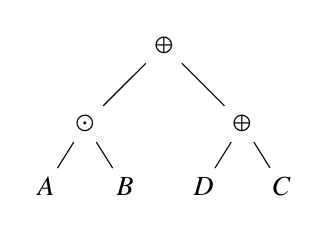
\begin{tikzpicture}[]
    \def\dx{0};
    \def\a{1.0};
    \def\b{0.5};
    \def\ya{-1.0};
    \def\yb{-0.8};
    \node[] at (\dx, 0) (P1) {$\oplus$};
    \node[] at (\dx+\a, \ya) (P2) {$\oplus$};
    \node[] at (\dx-\a, \ya) (M1) {$\odot$};
    \node[] at (\dx-\a-\b, \ya+\yb) (A) {$A$};
    \node[] at (\dx-\a+\b, \ya+\yb) (B) {$B$};
    \node[] at (\dx+\a+\b, \ya+\yb) (C) {$C$};
    \node[] at (\dx+\a-\b, \ya+\yb) (D) {$D$};
    \draw[] (P1) -- (M1);
    \draw[] (P1) -- (P2);
    \draw[] (P2) -- (C);
    \draw[] (P2) -- (D);
    \draw[] (M1) -- (A);
    \draw[] (M1) -- (B);
\end{tikzpicture}}

The left and right sibling of root node have size $|A|\times |B|$ and $|C|+|D|$ respectively.
Since the root node has type \texttt{SUM}, its size can be computed as $|A|\times |B| + |C|+|D|$.
One can compute the sizes of $A, B, C$ and $D$ recursively until the program meets either a the \texttt{LEAF} node or a \texttt{ZERO} node, which has a known size of $1$ or $0$ respectively.
\end{example}

\section{Weighted graphs}\label{sec:weighted}
All the previous discussion for unweighted graphs still holds for integer weighted graphs,
while for general weighted graphs, the independence polynomial is not well defined anymore.
For general weighted graphs, we are more interested to know the $k$ most weighted sets and their sizes.
Hence we define the extended tropical numbers as a natural generalization of tropical numbers:

\begin{equation}
\eqname{T$k$}
\begin{split}
    s \oplus t &= \texttt{largest}(s \cup t, k)\\
    s \odot t &= \texttt{largest}(\{a+b| a \in s, b\in t\}, k)\\
    \mymathbb{0} &= -\infty^{\otimes k}\\
    \mymathbb{1} &= -\infty^{\otimes k-1} \otimes 0
\end{split}\label{eq:ext-tropical}
\end{equation}
where $\texttt{largest}(s, k)$ means truncating the set by only keeping $k$ largest values in the set $s$.
The computation of $s \odot t$ is a maximum sum combination problem which can be done in time $\sim k\log(k)$.
One can find an efficient algorithm in \App{sec:maxsum}.
The vertex tensor and edge tensor become
\begin{equation}
    W^{{\rm T}k}(-\infty^{\otimes k-1} \otimes 1, w_v) = \left(\begin{matrix}
        \mymathbb{1} \\
        -\infty^{\otimes k-1} \otimes w_v
    \end{matrix}\right),   
    \qquad
        B^{{\rm T}k} = \left(\begin{matrix}
        \mymathbb{1}  & \mymathbb{1} \\
        \mymathbb{1} & \mymathbb{0}
    \end{matrix}\right),
\end{equation}
where we have used the relation $(-\infty^{\otimes k-1} \otimes 1)^{w_v} = -\infty^{\otimes k-1} \otimes w_v$.
Similar to the tropical numbers, we can combine the extended tropical algebra with a bit string sampler (\Eq{eq:singleconfig}) for finding the configuration of each size.
Since the $\odot$ operation of configuration sampler is not used, the resulting configurations are deterministic and complete.

\section{Performance benchmarks}\label{sec:benchmark}
We run a single thread benchmark on CPU Intel(R) Xeon(R) CPU E5-2686 v4 @ 2.30GHz,
and its CUDA version on a GPU Tesla V100-SXM2 16G.
The results are summarized in Figure~\ref{fig:benchmark}.
The graphs that we use in benchmarks are random three regular graphs,
 a typical type of sparse graphs that have a small treewidth that asymptotically smaller than $|V|/6$~\cite{Fomin2006}.
In this benchmark, we do not include traditional algorithms for finding the MIS size such as the branching algorithms~\cite{Tarjan1977, Robson1986} or dynamic programming based algorithms~\cite{Courcelle1990, Fomin2013},
because to the best of our knowledge, most of the properties mentioned in this paper are not computable within these frameworks.
The main goal of this section is to show the relative timing for computing different properties.

\begin{figure} 
    \centering
    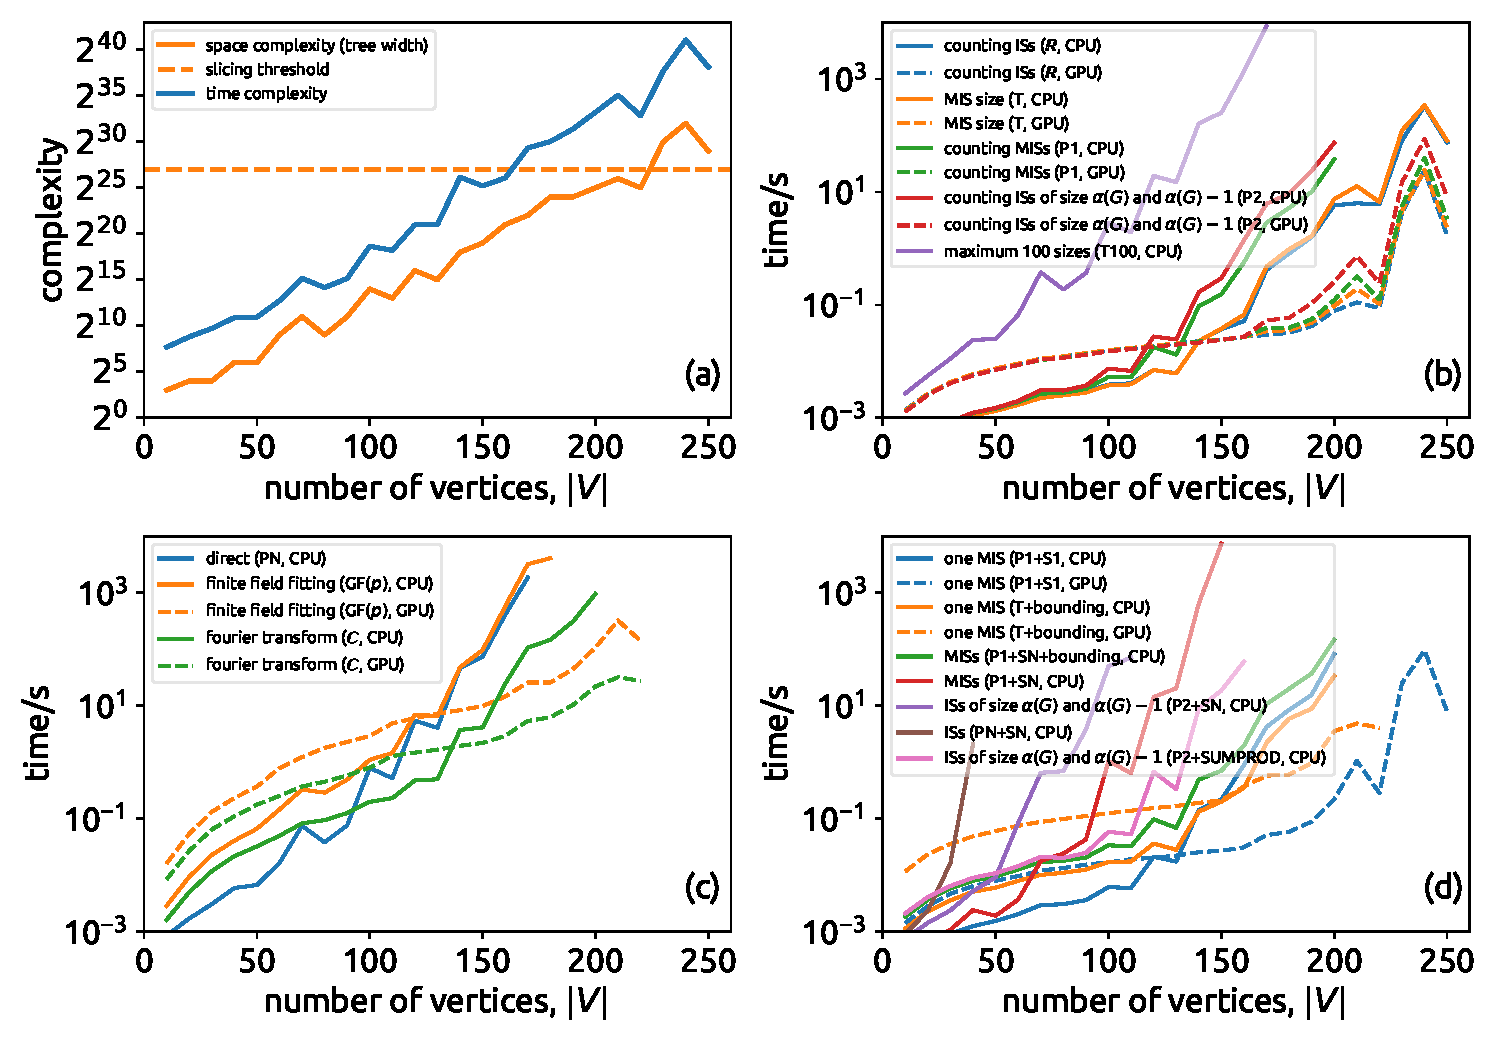
\includegraphics[width=\textwidth, trim={0cm 0cm 0cm 0cm}, clip]{figures/fig1.pdf}
    \caption{Benchmark results for computing different properties of independent sets of a random three regular graph with different tensor element types.
    The time in these plots only includes tensor network contraction, without taking into account the contraction order finding and just-in-time compilation time.
    Legends are properties, algebra and devices that we used in the computation; one can find the corresponding computed solution space property in \Tbl{tbl:generictypes}.
    (a) time and space complexity versus the number of vertices for the benchmarked graphs.
    (b) The computing time for calculating the MIS size and for counting of the number of all independent sets (ISs), the number of MISs,
        the number of independent sets having size $\alpha(G)$ and $\alpha(G)-1$, and finding $100$ largest sets sizes.
    (c) The computing time for calculating the independence polynomials with different approaches.
    (d) The computing time for configuration enumeration, including the enumeration of all independent set configurations, a single MIS configuration, all MIS configurations,
    all independent set configurations having size $\alpha(G)$ and $\alpha(G)-1$, and all independent set configurations having size $\alpha(G)$ and $\alpha(G)-1$ in the sum-product expression tree format,
    with or without bounding the enumeration space.
    }
    \label{fig:benchmark}
\end{figure}

Figure~\ref{fig:benchmark}(a) shows the time and space complexity of tensor network contraction for different graph sizes,
where the space complexity is the same as the treewidth of the problem graph.
Here, we assume our contraction order finding program has been converged to the optimal treewidth.
The contraction order is obtained using the local search algorithm in Ref.~\cite{Kalachev2021}.
In practice, slicing technique~\cite{Kalachev2021} is used for graphs with treewidth greater than 27 to fit the computation into a 16GB memory.
One can see that all the computing times in figure~\ref{fig:benchmark}(b), (c) and (d) have a strong correlation with the treewidth,
while in panel (d), the timing of certain computing tasks also strongly correlates with other factors like the configuration space size.
Among these benchmarks, computational tasks with data types tropical number of on CPU and real and complex numbers on both CPU and GPU can utilize fast basic linear algebra subprograms (BLAS) functions to evaluate tensor contractions, hence 
are much faster comparing to non-BLAS element types in the same category.
GPU computes much faster than CPU in all cases when the problem scale is large enough such that the actual computing time is comparable or larger than the launching overhead of CUDA kernels.
Most algebras can be computed on a GPU, except those requiring dynamic sized structures, i.e.\ types with algebra defined in \Eq{eq:polynomial}, \Eq{eq:set}, \Eq{eq:ext-tropical} and \Eq{eq:expr}.
In figure~\ref{fig:benchmark}(c), one can see the Fourier transformation based method is the fastest in computing the independence polynomial,
but it may suffer from round-off errors (\App{sec:fft}). The finite field (GF$(p)$) approach is the only method that does not have round-off errors and can be run on a GPU.
In figure~\ref{fig:benchmark}(d), one can see the technique to bound the enumeration space improves the performance for more than one order of magnitude in enumerating the MISs.
Bounding can also reduce the memory usage significantly, without which the largest computable graph size is only $\sim150$ on a device with 32GB main memory.

\section{Example case studies} \label{sec:examples}
In this section, we give a few examples where the different properties of independence sets are used.

\subsection{Number of independent sets and entropy constant for some hardcore lattice gases}\label{sec:entropy}
We compute the counting of all independent sets for graphs shown in Figure~\ref{fig:lattices}, where vertices are all placed on square lattices with lattice dimensions $L \times L$.
The types of graphs include: the square lattice graphs (Figure~\ref{fig:lattices}(a)); the square lattice graphs with a filling factor $p=0.8$, which means $\lfloor pL^{2} \rceil$ square lattices are occupied with vertices  (Figure~\ref{fig:lattices}(b));
the King's graphs  (Figure~\ref{fig:lattices}(c)); the King's graphs with a filling factor $p = 0.8$  (Figure~\ref{fig:lattices}(d)).
The number of independent sets for square lattice graphs of size $L \times L$ form a well-known integer sequence (\href{https://oeis.org/A006506}{OEIS A006506}), which is thought as a two-dimensional generalization of the Fibonacci numbers.
We computed the integer sequence for $L=38$ and $L=39$, which, to the best of our knowledge, is not known before.
In the computation, we used the finite-field algebra for contracting arbitrarily high precision integer tensor networks. 

A theoretically interesting number that can be computed using the number of independent sets is the entropy constant for the hardcore lattice gases on these graphs, which can tell us thermal dynamic properties of these lattices at the high temperature limit.
For the square lattice graphs, it is called the \textit{hard square entropy constant} (\href{https://oeis.org/A085850}{OEIS A085850}), which is defined as $\lim_{L\rightarrow \infty} F(L,L)^{1/L^2}$, where $F(L,L)$ is the number of independent sets of a given lattice dimensions $L \times L$. This quantity arises in statistical mechanics of hard-square lattice gases~\cite{Baxter1980, Pearce1988} and is used to understand phase transitions for these systems. This entropy constant is not known to have an exact representation, but it is accurately known in many digits. Similarly, we can define entropy constants for other lattice gases. In \Fig{fig:hardsquare}, we look at how $F(L,L)^{1/\lfloor pL^2\rceil}$ scales as a function of the grid size $L$ for all types of graphs shown in Figure~\ref{fig:lattices}. Our results match the known results for the non-disordered square lattice and King's graphs. For disordered square lattice and King's graphs with a filling factor $p=0.8$, we randomly sample 1000 graph instances. To our knowledge, the entropy constants for these disordered graphs have not been studied before. Interestingly, the variations due to different random instances are negligible for this entropy quantity. 

\begin{figure}[t] 
    \centering
    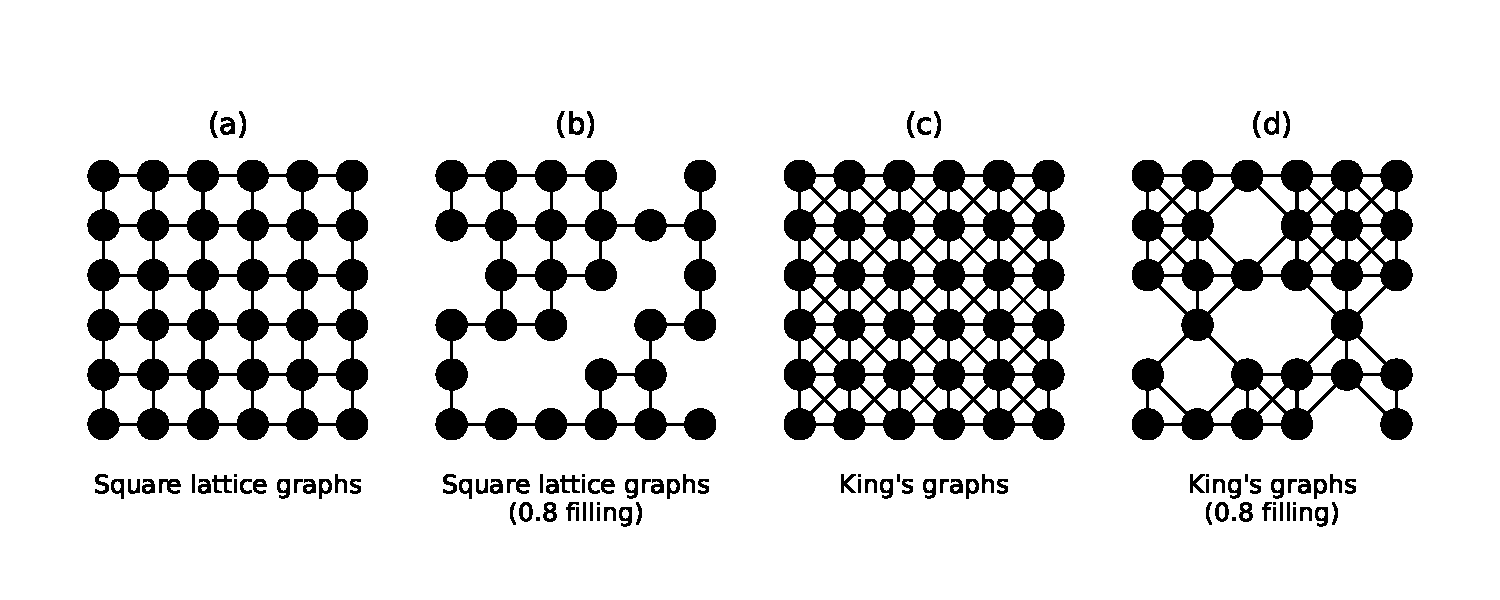
\includegraphics[width=\textwidth, trim={0cm 1cm 0cm 1cm}, clip]{figures/lattices.pdf}
    \caption{The types of graphs used in the case study in section \ref{sec:entropy}.
    The lattice dimensions are $L\times L$. (a) square lattice graphs. (b) square lattice graphs with a filling factor $p=0.8$.
    (c) King's graphs. (d) King's graphs with a filling factor $p=0.8$.}
    \label{fig:lattices}
\end{figure}

\begin{figure}[t] 
    \centering
    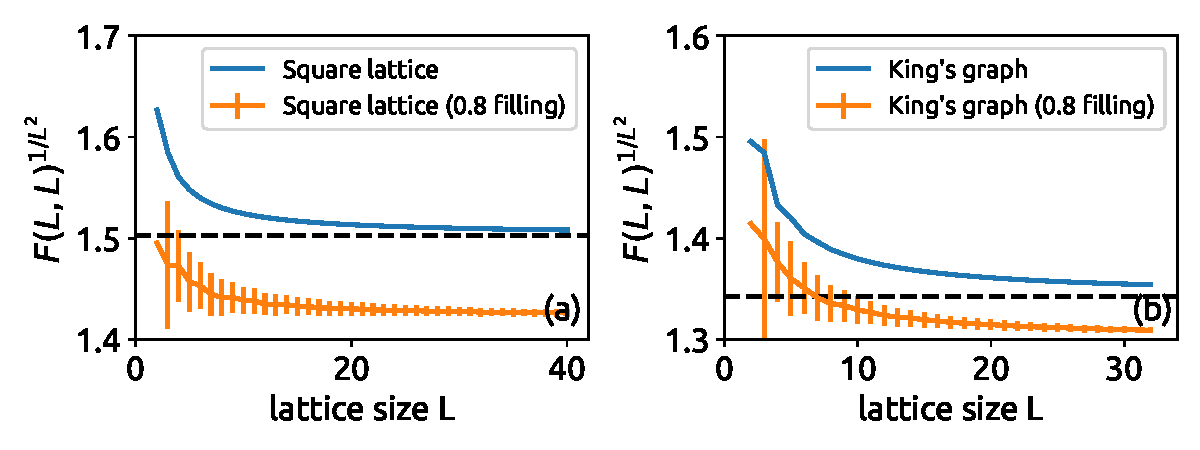
\includegraphics[width=\textwidth, trim={0cm 0cm 0cm 0cm}, clip]{figures/fig5.pdf}
    \caption{Mean entropy for lattice gases on graphs defined in \Fig{fig:lattices}.
    We sampled $1000$ instances for $p=0.8$ lattices and the error bar is too small to be visible.
    The horizontal black dashed lines are for $\lim_{L\rightarrow \infty} F(L,L)^{1/L^2}$ for the corresponding non-disordered square lattice and King's graphs.
    }
    \label{fig:hardsquare}
\end{figure}

\subsection{The Overlap Gap Property\label{sec:overlap-gap}}
With the tool to enumerate configurations, one can %try to 
understand the structure of the independent set configuration space,
such as the optimization landscape for finding the MISs.
One of the known barriers for finding the MIS is the so-called Overlap Gap Property~\cite{Gamarnik2013, Gamarnik2019}.
Intuitively, if the Overlap Gap Property is present, it means every two large independent sets either have a significant intersection or very small intersection;
it implies that large independent sets are clustered together. \purple{Do you want me to write a more formal definition as well or do you think it's not necessary?}\blue{I suppose you want to justify the origin of ``ratio'', then it would great if you can explain it more clearly. However, explaining the concept overlap gap property well seems to be impossible in a this paper (you need at least some plots).}
This clustering property has been used to rigorously prove upper bounds on the performance of local algorithms~\cite{Gamarnik2013, Gamarnik2019}.
It was shown that for finding MISs of $d$-regular graphs with $d$ and graph sizes both being large, there exists Overlap Gap Property~\cite{Rahman2017,Gamarnik2021}.
However, it is not known whether for small $d$, e.g. $3$- regular graphs, this statement is still true.
Here, we direct sample from the computed configurations of large independent sets to investigate the presence or absence of the Overlap Gap Property for some given graphs.
%We do not explore the full configurations space because the
Because the number of configurations is too large to fit into storage, we use the compact sum-product expression tree representation to sample from independent sets of a given size. 
We compare  nine randomly generated instances from two categories of graphs: King's graphs at $\rho = 0.8$ filling and $3$-regular graphs.% that we want to investigate.
%Each category contains nine randomly generated instances, due to the limitation of computing resources,
Our method can sample from independent sets of King's graph up to $20\times 20$ ($320$ vertices) and the size of $3$-regular graphs are $110$.
In particular, in \Fig{fig:hamming}, 
we sample two sets of $10^4$ configurations from the ISs at sizes $\geq \lfloor (1-\text{ratio}) \times \alpha(G)\rfloor$ for each instance
 and show the pairwise Hamming distance distribution for the enumerated configurations.
In \Fig{fig:hamming}(a), we observed a clear single peak structure at a fixed distance normalized by the MIS size for the King's graphs.
Which is a clear evidence of the absence of the Overlap Gap Property in $0.8$ filling King's graph.
Given the fact that the MIS problem on an arbitrary graph can be mapped to a King's graph at a certain filling~\cite{Ebadi2022}, this result is highly nontrivial.
While in \Fig{fig:hamming}(b), we observed the multiple peak structure in $3$-regular graphs as the ratio becomes small.
This indicates the presence of the Overlap Gap Property \blue{@Maddie, I am not sure if we can say ``indicates the presence of the Overlap Gap Property'' here because it is so different from the official definition of OGP, I want to change it to ``disconnected clusters exist in the configuration space for large independent sets, however, it requires further study to show whether 3-regular graphs have the overlap gap property or not.'', which one do you think is more correct?} and disconnected clusters exist in the configuration space for large independent sets.
We expect our numerical tool can be used to understand this phenomenon better and to further investigate the graph properties and the geometry of the configuration spaces for a variety of graph instances.
\begin{figure} 
    % \begin{subfigure}[t]{\textwidth}
    %     \centering
    %     %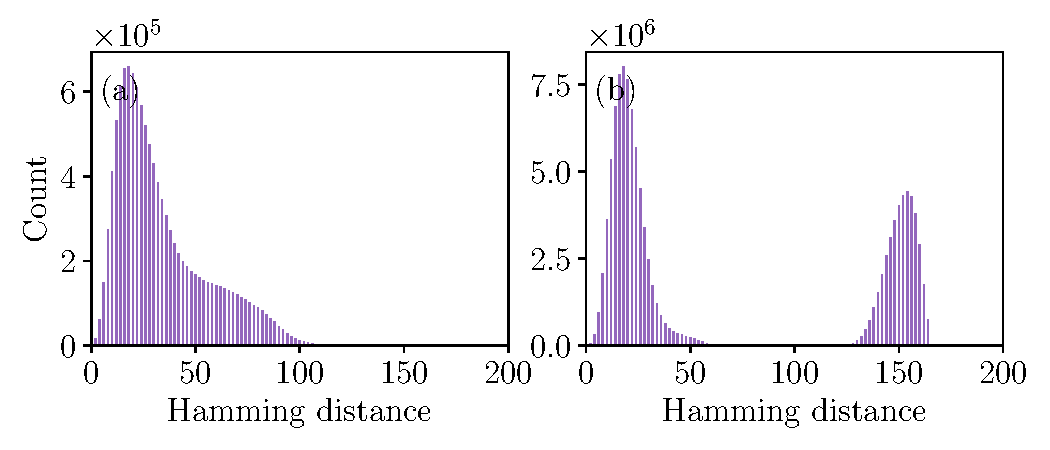
\includegraphics[width=\textwidth, trim={0cm 0cm 0cm 0cm}, clip]{figures/fig3.pdf}
    %     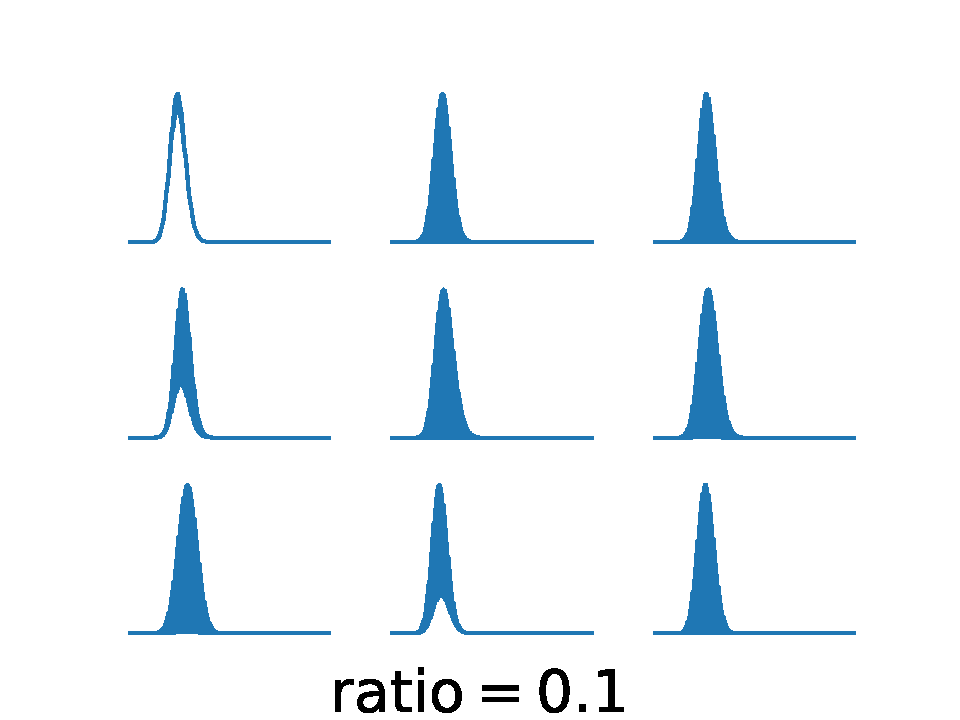
\includegraphics[width=0.3\textwidth, trim={0.5cm 0cm 0.5cm 1cm}, clip]{figures/grid-diag-size20d3-k3-alpha0.1-n10000.pdf}
    %     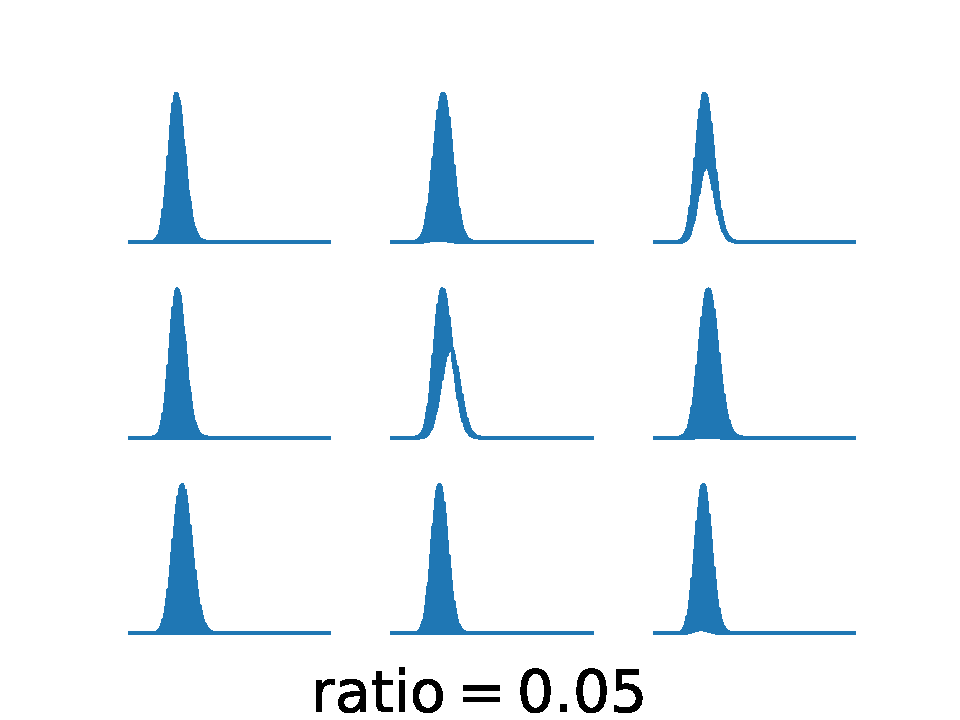
\includegraphics[width=0.3\textwidth, trim={0.5cm 0cm 0.5cm 1cm}, clip]{figures/grid-diag-size20d3-k3-alpha0.05-n10000.pdf}
    %     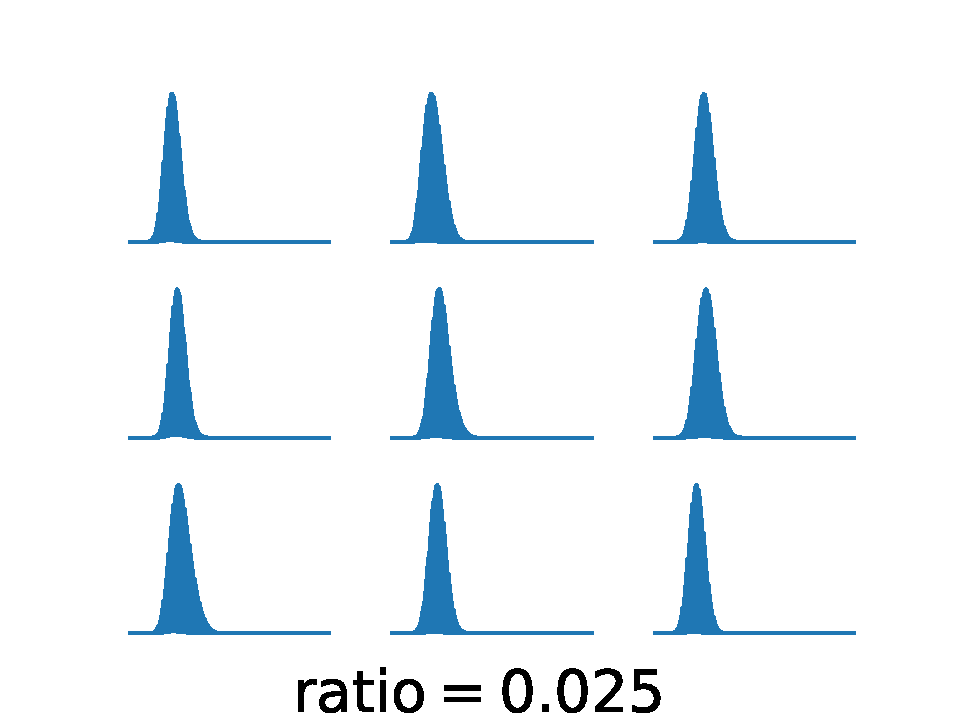
\includegraphics[width=0.3\textwidth, trim={0.5cm 0cm 0.5cm 1cm}, clip]{figures/grid-diag-size20d3-k3-alpha0.025-n10000.pdf}
    %     \caption{Nine King's graphs of size $20\times 20$, $0.8$ filling.}
    % \end{subfigure}
    % \begin{subfigure}[t]{\textwidth}
    %     \centering
    %     %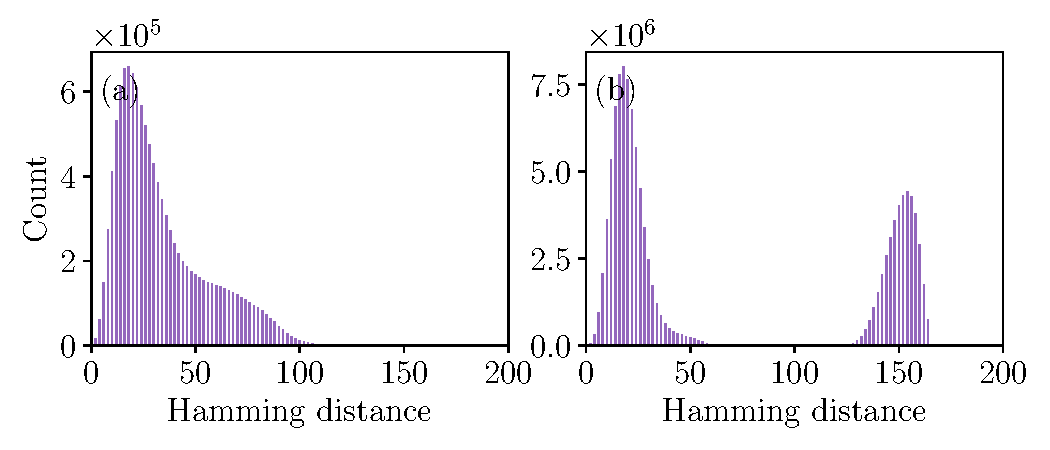
\includegraphics[width=\textwidth, trim={0cm 0cm 0cm 0cm}, clip]{figures/fig3.pdf}
    %     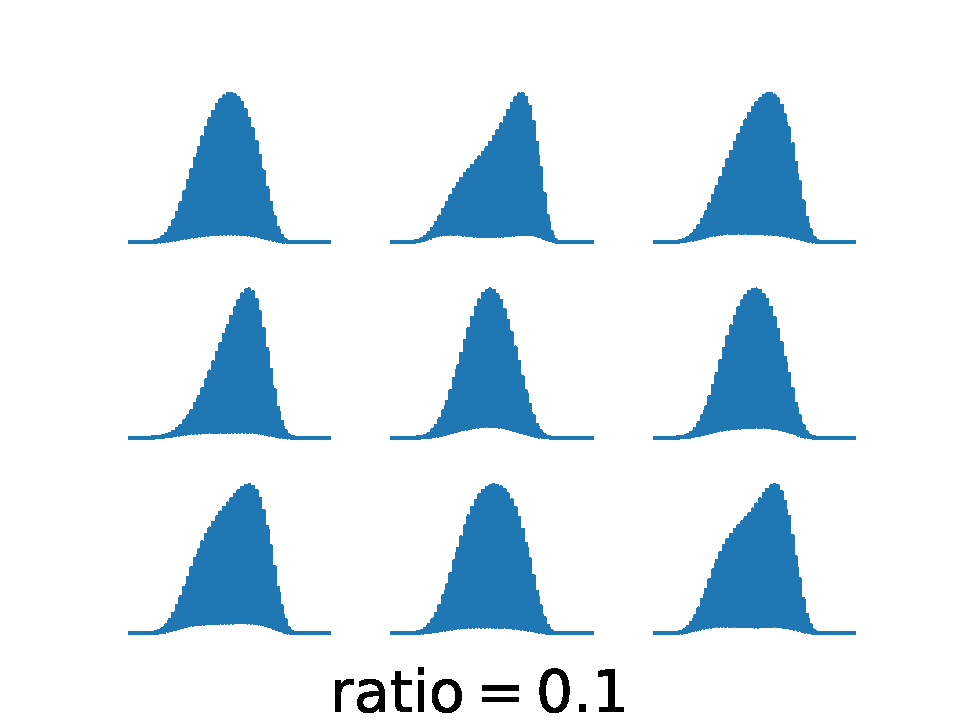
\includegraphics[width=0.3\textwidth, trim={0.5cm 0cm 0.5cm 1cm}, clip]{figures/grid-regular-size110d3-k3-alpha0.1-n10000.pdf}
    %     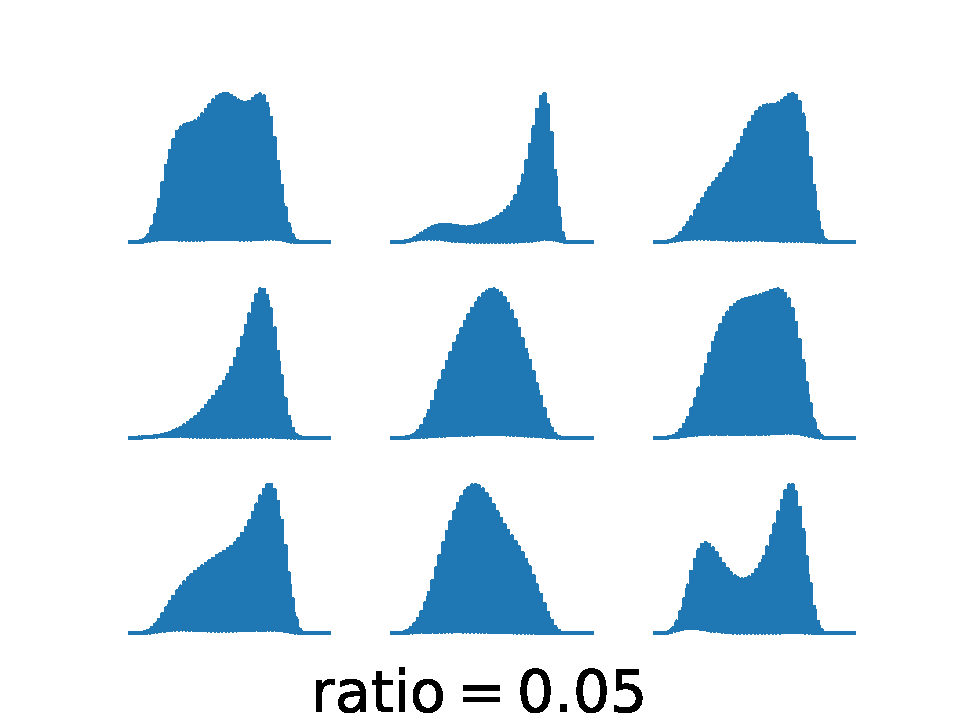
\includegraphics[width=0.3\textwidth, trim={0.5cm 0cm 0.5cm 1cm}, clip]{figures/grid-regular-size110d3-k3-alpha0.05-n10000.pdf}
    %     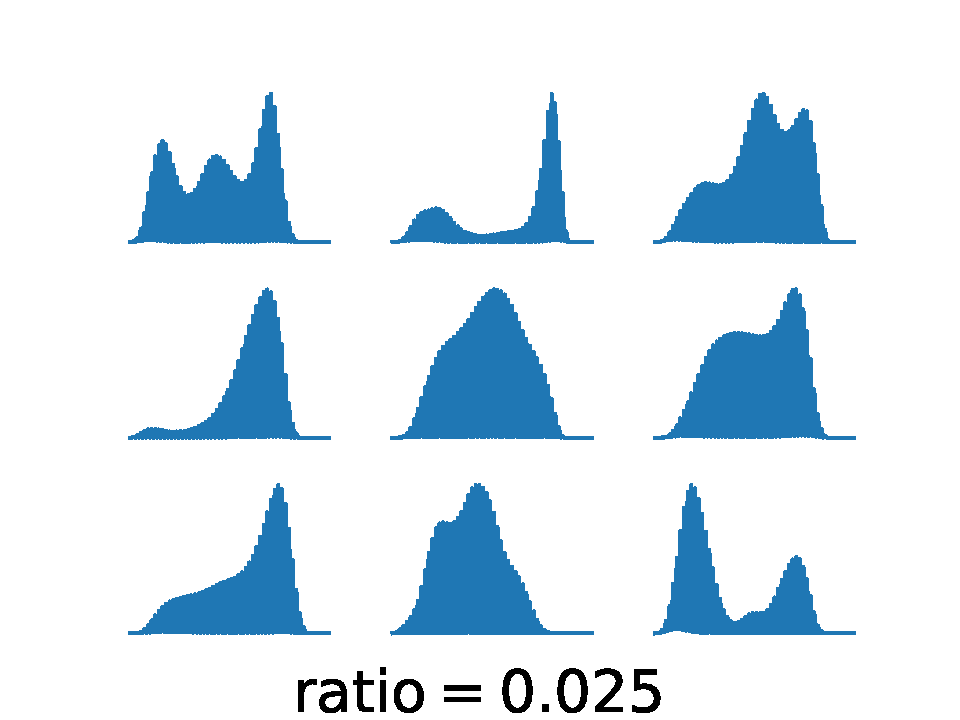
\includegraphics[width=0.3\textwidth, trim={0.5cm 0cm 0.5cm 1cm}, clip]{figures/grid-regular-size110d3-k3-alpha0.025-n10000.pdf}
    %     \caption{Nine random three regular graphs of size $110$.}
    % \end{subfigure}
    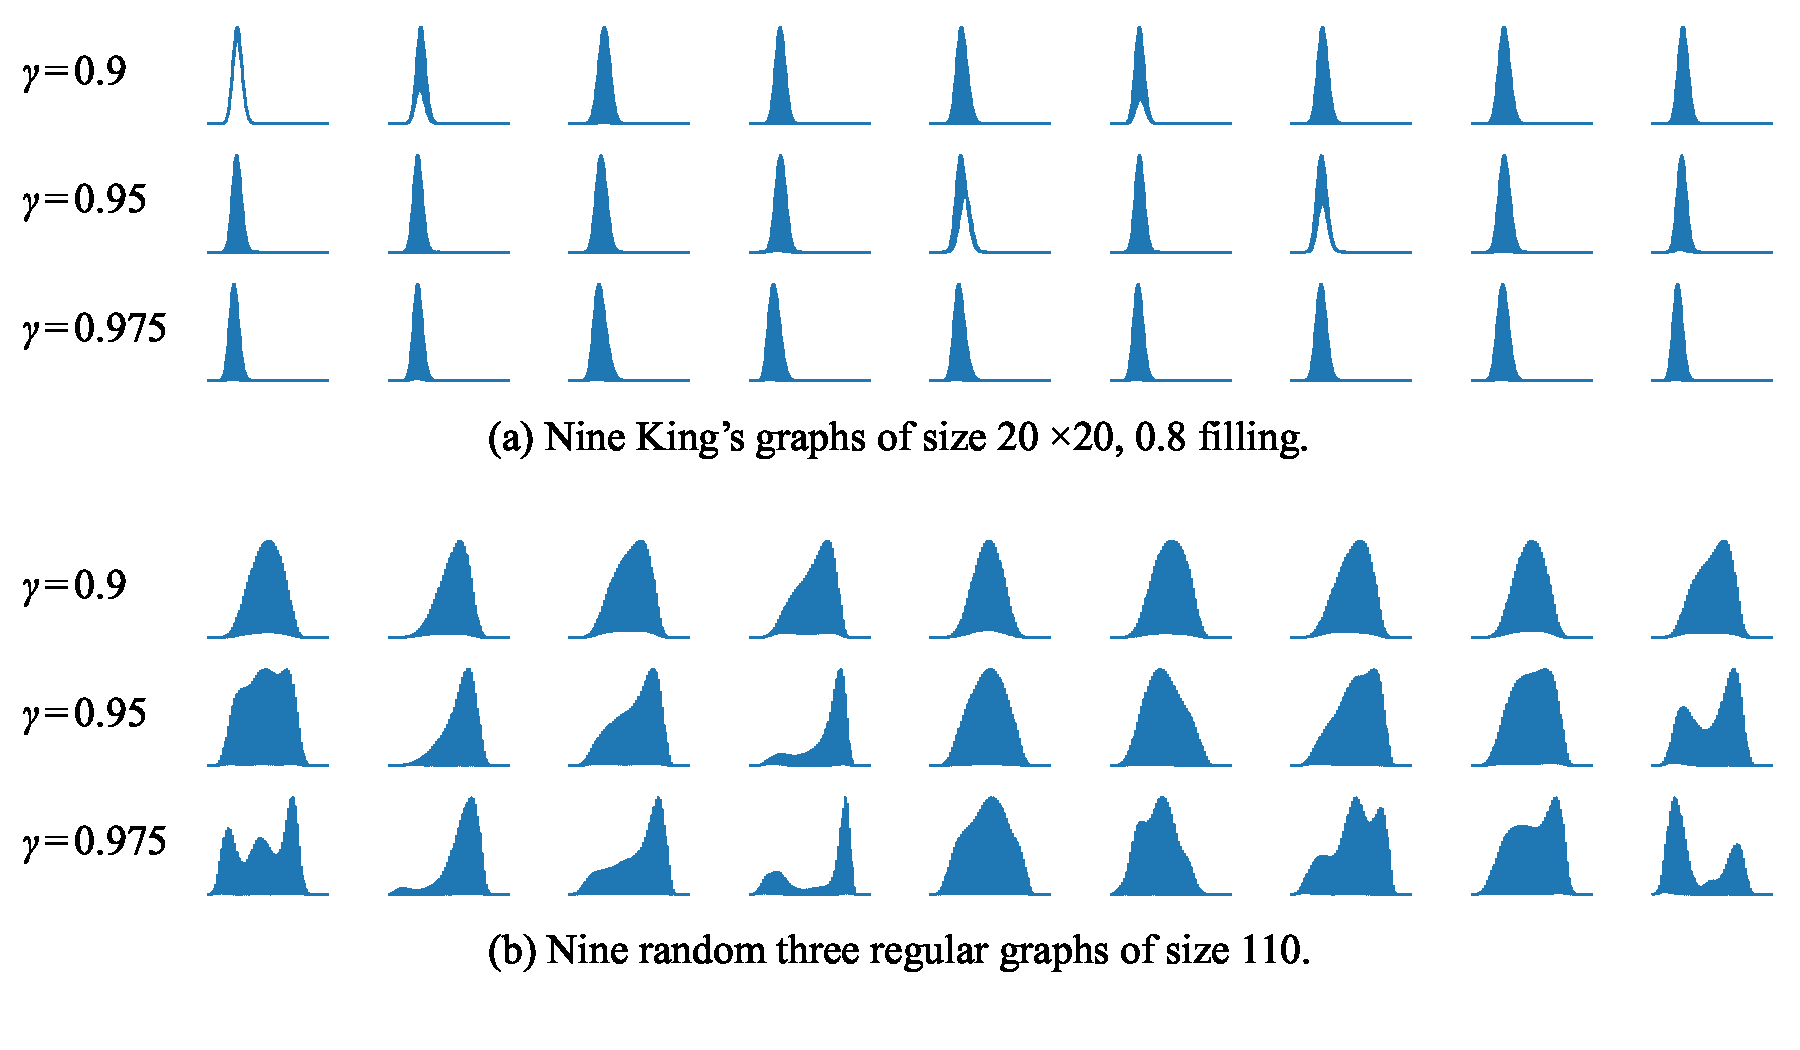
\includegraphics[width=\textwidth, trim={0.0cm 1cm 0.0cm 0cm}, clip]{figures/fig6.pdf}
    \caption{The plot of pairwise Hamming distances distribution for configurations sampled from independent sets with sizes $\geq \lfloor(1-{\rm ratio}) \times \alpha(G)\rfloor$.
    In each plot, the $x$-axis is the Hamming distance normalized by the total number of vertices and the $y$-axis is the probability.
    The ``filled'' region is caused by the fast oscillation of configuration populations of even and odd Hamming distances.
    }
    \label{fig:hamming}
\end{figure}

\subsection{Visualizing experimental quantum algorithm outputs for solving Maximum Independent Set}

\begin{figure} 
    \centering
    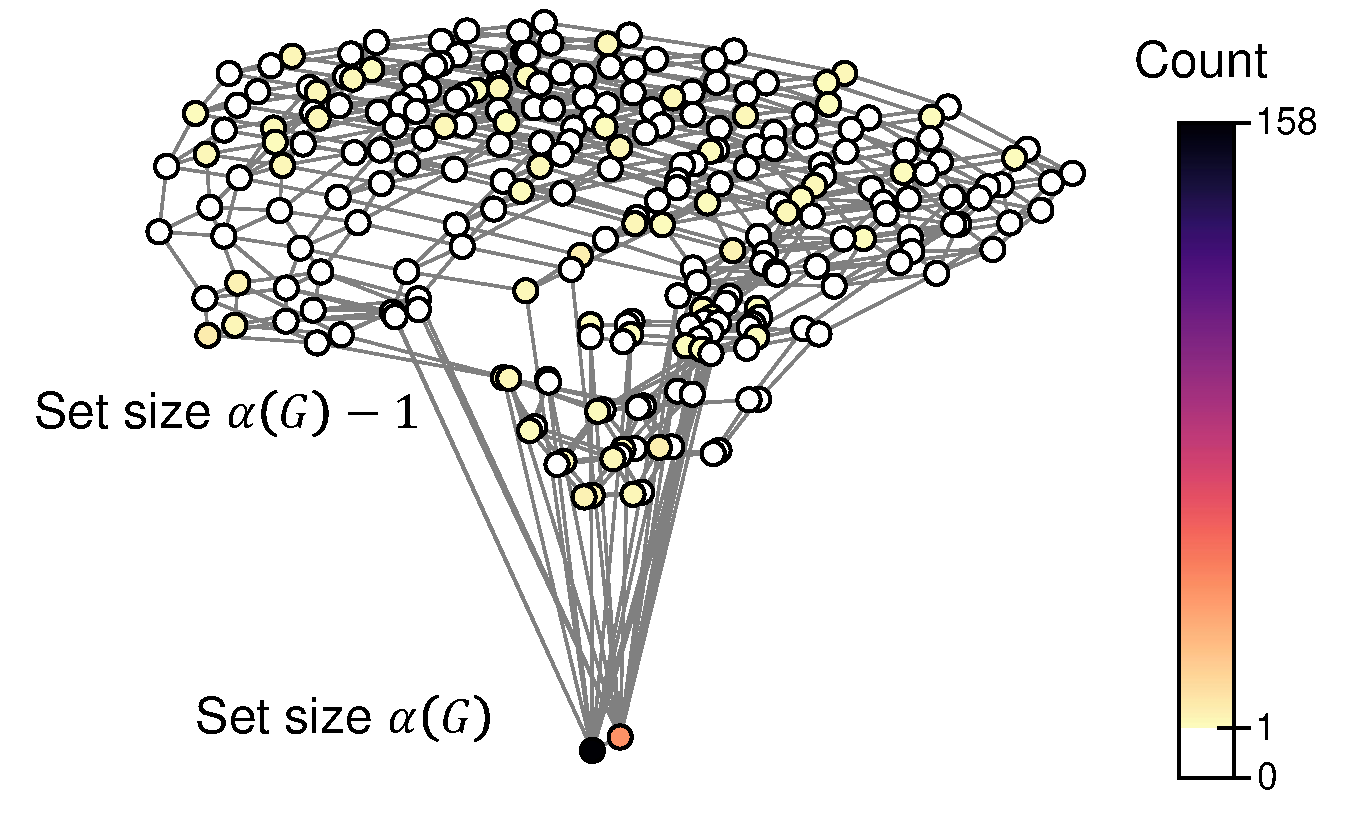
\includegraphics[width=.65\textwidth, trim={0cm 0cm 0cm 0cm}, clip]{figures/exp_configurations.pdf}
    \caption{A visualization of experimental outputs of a quantum algorithm for solving the maximum independent set problem.
    Each vertex represents an independent set, and each edge represents a pair of  independent sets that differ by a swap operation or a vertex addition.}
    \label{fig:exp_configuratoins}
\end{figure}
The ability to enumerate configurations can also be used to understand the distribution of outputs from algorithms for solving NP-hard combinatorial optimization problems.
This can give detailed insights to performance of the algorithm, such as if the algorithm is likely to return independent sets from certain clusters of local or global minima in the solution space.
As an example, we show in Figure~\ref{fig:exp_configuratoins} how our algorithm can be used to visualize experimental outputs of a quantum algorithm for solving the Maximum Independent Set problem using a programmable Rydberg atom array quantum computer~\cite{Ebadi2022}.
The structure of the solution space for a King's graph with $39$ vertices and filling factor $\rho=0.8$ can be visualized on a graph where each vertex represents a large independent set, and each edge represents a pair of  independent sets that differ by a swap operation or a vertex addition to the set.
The algorithm either finds the MIS with size $\alpha(G)$ with high probability, or returns a suboptimal independent set, usually with size $\alpha(G)-1.$
The algorithm does not appear to return solely local minima with large Hamming distance from the MISs as suggested by~\cite{altshuler2010}\blue{Fix ref.},
but samples from local minima with a wide range of Hamming distances from the MISs.
Consistent with Sec.~\ref{sec:overlap-gap}, there are no disconnected clusters in the solution space for this King's graph.


\section{Discussion and conclusion}
In this paper, we introduce a method to use generic programming and tensor networks to compute a number of different solution space properties of certain classes of NP-hard combinatorial optimization problems. % the maximum independent set problem. %, including the largest several independent sets sizes, the number of independent sets of a given size, and the enumeration of independent sets of a given size.
For each solution space property, we design a commutative semiring algebra for the tensor element type. By using the same tensor network but replacing the tensor network elements with elements of different algebras, we can compute different solution space properties. This technique can further be generalized to computing solution space properties beyond the examples given in this paper. % such as the largest several independent sets sizes, the number of independent sets of a given size, and the enumeration of independent sets of a given size.
%With different algebras, the contraction of the same tensor network gives us the different properties.
The different data types introduced in the main text to compute these properties are  summarized in the diagram in \Fig{fig:venn-diagram}. %We go beyond using real numbers and use polyn
Other than the case with real numbers, we have polynomials and truncated polynomials.
We combine them with the bit string algebra, the set algebra, and sum-product expression tree algebra for finding, enumerating, and sampling of independent sets at a given size. Three examples are shown to demonstrate how our method can be used to understand the solution space better.
In the first example, we show how our method can help computing the entropy constant for some hardcore lattice gases on 2D square lattices. We compute the 2D generalization of Fibonacci integer sequence up to size $39$, which is larger than the previous record $37$.
In the second example, we analyze the pairwise Hamming distances from configurations directly sampled from large independent sets of King's graphs at $0.8$ filling and three regular graphs. We show the strongest numeric evidence so far of the absence of Overlap Gap Property in King's graph and the existence of Overlap Gap properties in three regular graphs.
In the last example, we show how our algorithm helps people to understand the performance of a quantum variational algorithms on Rydberg atom arrays to find maximum independent sets. This is a research frontier that understanding which can help people design better quantum algorithms to beat its classical counterpart.
These algebras are of generic use: they can be utilized to compute properties of maximal independent sets and a variety of other combinatorial problems such as the matching problem, the k-coloring problem, the max-cut problem, and the set packing problem, as detailed in \App{sec:otherproblems}. 
%Moreover, since the independence polynomial is closely related to the matching polynomial~\cite{Levit2005}, the clique polynomial~\cite{Hoede1994}, and the vertex cover polynomial~\cite{Akbari2013},
%our algorithm to compute the independence polynomial can also be used to compute these graph polynomials.
By adapting to the style of generic programming, we can implement all the algorithms without much effort.
We show some of the Julia language implementations in Appendix~\ref{sec:technical}.
A complete implementation can be found in our Github repository~\cite{GraphTensorNetworks}. 
We expect our tool can be used to understand and study many interesting applications of independent sets and beyond. We also hope this approach of generic tensor networks can inspire future works on tensor network computations.

\section*{Acknowledgments}
We would like to thank Pan Zhang for sharing his python code for optimizing contraction orders of a tensor network.
We acknowledge Sepehr Ebadi and Leo Zhou for coming up with many interesting questions about independent sets and their questions strongly motivated the development of this project.
We thank Benjamin Schiffer for providing helpful feedback on the manuscript.
We thank Chris Elord for helping us write the fastest matrix multiplication library for tropical numbers, TropicalGEMM.jl. % he is a man of speed!
We would also like to thank a number of open-source software developers, including Roger Luo, Time Besard, Edward Scheinerman and Katharine Hyatt
for actively maintaining their packages and resolving related issues voluntarily.
\blue{funding information}

\bibliographystyle{siamplain}
\bibliography{refs}

\appendix

\section{An alternative way to construct the tensor network}\label{sec:energymodel}

Let us characterize the independent set problem on graph $G=(V, E)$ as an energy model
\begin{equation}\label{eq:eng}
    \mathcal{E}(G, s) = -\sum_{i\in V(G)} w_i s_i + \infty \sum_{\langle i,j\rangle \in E(G)}s_i s_j
\end{equation}
where $s_i$ is a spin on vertex $i \in V$ and $w_i$ is an onsite energy term associated with it.
The first term is the energy that corresponds to the inverse of the independent set size and the second term describes the independence contraint.
In physical systems, this contraint term usually corresponds to the Rydberg blockade~\cite{Pichler2018, Ebadi2022} in cold atom arrays or the repulsive force in hard core lattice model~\cite{Dyre2016, Fernandes2007}.
Its partition function is defined as
\begin{equation}\label{eq:partition}
    \begin{split}
    Z(G, \beta) = \sum_{s}e^{-\beta \mathcal{E}(G, s)} = \sum_{s\in \mathcal{I}(G)} e^{\beta \sum w_i s_i}\\
         = \sum_{k=0}^{\alpha(G)}a(k) e^{\beta k}  \qquad \quad (k = \sum w_i s_i)
    \end{split}
\end{equation}
where $\mathcal{I}(G)$ is the set of independent sets of graph $G$.
$\alpha(G)$ is the absolute value of the minimum energy (maximum independent set size).
$a(k)$ is the number of spin configurations with energy $-k$ (independent sets of size $k$).
The partition function can be evaluated as a tensor network contraction,
where the tensor network is constructed by placing a vertex tensor on each spin $i$
\begin{equation}
    W(\beta, w_i) = \left(\begin{matrix}
        1 \\
        e^{\beta w_i}
    \end{matrix}\right),
\end{equation}
and an edge tensor on each bond
\begin{equation}
       B = \left(\begin{matrix}
        1  & 1\\
        1 & 0
    \end{matrix}\right),
\end{equation}
where the $0$ in the bond tensor coming from $e^{-\beta\infty}$ in the second term of \Eq{eq:eng}.
By letting $x = e^{\beta}$, we get the tensor network for computing the independence polynomial as described by \Eq{eq:vertextensor} and \Eq{eq:edgetensor},
and by letting $w_i=1$, the second line of \Eq{eq:partition} is the independence polynomial.

\section{An example of contraction complexity increase due to introducing $\delta$ tensors}\label{sec:tensorbad}
As we have mentioned in the main text,
a standard tensor network notation is equivalent to the generalized tensor network by introducing $\delta$ tensors,
where a $\delta$ tensor of rank $d$ is defined as
\begin{equation}
    \delta_{i_1, i_2,\ldots,i_d} = \begin{cases}
        1, & i_1=i_2=\ldots =i_d,\\
        0, & \text{otherwise}.
    \end{cases}
\end{equation}

In the following, we are going to show introducing $\delta$ tensors might increase the contraction complexity of a tensor network.
Let us consider the following King's graph.

\centerline{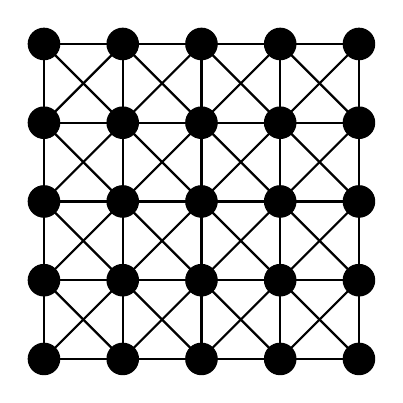
\begin{tikzpicture}
    \def\r{0.2}
    \foreach \x in {1,...,5}
        \foreach \y in {1,...,5}
            \filldraw[fill=black] (\x,\y) circle [radius=\r];
    \foreach \x in {1,...,5}
        \foreach \y in {1,...,4}{
            \draw [black,thick] (\x,\y) -- (\x,\y+1);
            \draw [black,thick] (\y,\x) -- (\y+1,\x);
        }
    \foreach \x in {1,...,4}
        \foreach \y in {1,...,4}{
            \draw [black,thick] (\x,\y) -- (\x+1,\y+1);
            \draw [black,thick] (\y+1,\x) -- (\y,\x+1);
        }
\end{tikzpicture}}

By mapping the independent set problem to a standard tensor network with $\delta$ tensors,
we have the following graphical representation.

\centerline{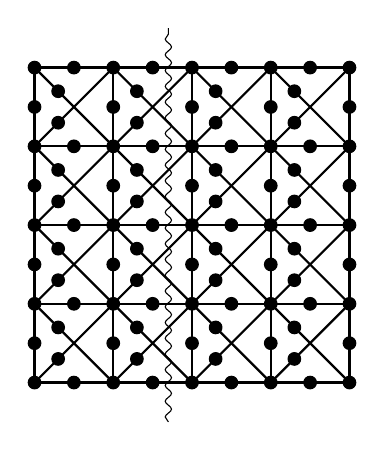
\begin{tikzpicture}
    \def\r{0.08}
    \def\a{0.1}
    \foreach \x in {1,...,5}
        \foreach \y in {1,...,5}
            \filldraw[fill=black] (\x,\y) circle [radius=\r];
    \foreach \x in {1,...,5}
        \foreach \y in {1,...,4}{
            \filldraw[fill=black] (\x,\y+0.5) circle [radius=\r];
            \filldraw[fill=black] (\y+0.5,\x) circle [radius=\r];
            \draw [black,thick] (\x,\y) -- (\x,\y+1);
            \draw [black,thick] (\y,\x) -- (\y+1,\x);
        }
    \foreach \x in {1,...,4}
        \foreach \y in {1,...,4}{
            \filldraw[fill=black] (\x+0.3,\y+0.3) circle [radius=\r];
            \filldraw[fill=black] (\y+0.3,\x+0.7) circle [radius=\r];
            \draw [black,thick] (\x,\y) -- (\x+1,\y+1);
            \draw [black,thick] (\y+1,\x) -- (\y,\x+1);
        }
    \tikzset{decoration={snake,amplitude=.4mm,segment length=2mm,
                    post length=0mm,pre length=0mm}}
    \draw [decorate] (2.7, 0.5) -- (2.7, 5.5);
\end{tikzpicture}}

In this diagram, the circle on each vertex in the original graph is a $\delta$ tensor of rank $8$ or less.
If we contract this tensor network in a naive column-wise order, the maximum intermediate tensor has rank $\sim3L$, requiring a storage of size $\approx 2^{3L}$.
If we relax the restriction that each label must appears exactly twice, we have the following hypergraph representation of a generalized tensor network.

\centerline{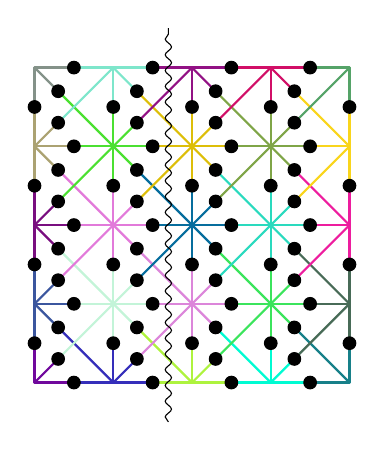
\begin{tikzpicture}
    \def\r{0.08}
    \def\a{0.07}
    \def\L{0.6}
    \def\l{0.1}
    \def\sql{0.24}
    \pgfmathsetseed{2}
    \foreach[evaluate={\cr=0.1+0.5*Mod(\x,2)}] \x in {1,...,5}
        \foreach[evaluate={\cg=0.1+0.3*Mod(\y,2); \cy=0.5-0.5*Mod(\y,2)}] \y in {1,...,5}{
            \edef\R{\pdfuniformdeviate 255}
            \edef\G{\pdfuniformdeviate 255}
            \edef\B{\pdfuniformdeviate 255}
            \xdefinecolor{MyColor}{RGB}{\R,\G,\B}
            \ifnum \x < 5
                \draw [thick, MyColor, opacity=1.0, line cap=round] (\x,\y) -- (\x+0.5,\y);
                \ifnum \y < 5
                \draw [thick, MyColor, opacity=1.0, line cap=round] (\x,\y) -- (\x+0.3,\y+0.3);
                \fi
                \ifnum \y > 1
                \draw [thick, MyColor, opacity=1.0, line cap=round] (\x,\y) -- (\x+0.3,\y-0.3);
                \fi
            \fi
            \ifnum \x > 1
                \draw [thick, MyColor, opacity=1.0, line cap=round] (\x,\y) -- (\x-0.5,\y);
                \ifnum \y < 5
                \draw [thick, MyColor, opacity=1.0, line cap=round] (\x,\y) -- (\x-0.7,\y+0.7);
                \fi
                \ifnum \y > 1
                \draw [thick, MyColor, opacity=1.0, line cap=round] (\x,\y) -- (\x-0.7,\y-0.7);
                \fi
            \fi
            \ifnum \y < 5
                \draw [thick, MyColor, opacity=1.0, line cap=round] (\x,\y) -- (\x,\y+0.5);
            \fi
            \ifnum \y > 1
                \draw [thick, MyColor, opacity=1.0, line cap=round] (\x,\y) -- (\x,\y-0.5);
            \fi
        }
    \foreach \x in {1,...,5}
        \foreach \y in {1,...,5}{
            %\filldraw[fill=black] (\x,\y) circle [radius=0.7*\r];
        }
    \foreach \x in {1,...,5}
        \foreach \y in {1,...,5}{
            \ifnum \y < 5
                \filldraw[fill=black] (\x,\y+0.5) circle [radius=\r];
                \filldraw[fill=black] (\y+0.5,\x) circle [radius=\r];
            \fi
        }
    \foreach \x in {1,...,4}
        \foreach \y in {1,...,4}{
            \filldraw[fill=black] (\x+0.3,\y+0.3) circle [radius=\r];
            \filldraw[fill=black] (\y+0.3,\x+0.7) circle [radius=\r];
        }
    \tikzset{decoration={snake,amplitude=.4mm,segment length=2mm,
                    post length=0mm,pre length=0mm}}
    \draw [decorate] (2.7, 0.5) -- (2.7, 5.5);
\end{tikzpicture}}
Here, we use different colors to distinguish different hyperedges.
A vertex tensor always has rank $1$ and is not shown here since it does not change the contraction complexity.
If we contract this tensor network in the column-wise order, the maximum intermediate tensor rank is $\sim L$, which can be seen by counting the number of colors at the cut.

\section{Hard problems and tensor networks}\label{sec:otherproblems}
\subsection{Maximal independent sets and maximal cliques}\label{sec:maximal}
Since finding maximal cliques of a graph is equivalent to finding the maximal independent sets of its complement graph, in the following,
we limit our discussion to finding maximal independent sets.
Let us denote the neighborhood of a vertex $v$ as $N(v)$ and the closed neighborhood of $v$ as $N[v] = N(v)\cup \{v\}$.
A maximal independent set $I_m$ is an independent set where there does exist a vertex $v \in V$ such that $I_m \cap N[v]  = \emptyset$,
i.e. an independent set that can not become a larger one by adding a new vertex.
To characterize the maximal independence restriction, one can quantify over a local set $N[v]$ with a local tensor:
\begin{equation}\label{eq:maximal}
    T(x_v, w_v)_{s_1,s_2,\ldots,s_{|N(v)|},s_v} = \begin{cases}
        s_vx_v^{w_v} & s_1=s_2=\ldots=s_{|N(v)|}=0,\\
        1-s_v& \text{otherwise}.\\
    \end{cases}
\end{equation}
Intuitively, it means if all the neighbourhood vertices are not in $I_{m}$, i.e., $ s_1=s_2=\ldots=s_{|N(v)|}=0$, then $v$ should be in $I_{m}$ and contribute a factor $x_{v}$,
otherwise, if any of the neighbourhood vertices is in $I_{m}$, then $v$ cannot be in $I_{m}$.
As an example, for a vertex of degree 2, the resulting rank-3 tensor is
\begin{equation}
    T(x_v, w_v)=\left(\begin{matrix}
    \left(\begin{matrix}
        ~~0 &~1 \\
        ~~1 &~1
    \end{matrix}\right)\\
    \left(\begin{matrix}
        x_v^{w_v} &0 \\
        0 &0
    \end{matrix}\right)
    \end{matrix}\right).
\end{equation}
 
Let us consider the example in~\Sec{eg:tensorcontraction}: its corresponding tensor network structure for computing the maximal independent polynomial becomes

    \centerline{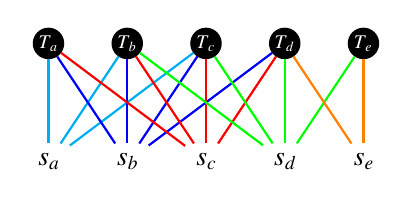
\begin{tikzpicture}[
    dot/.style = {circle, fill, minimum size=#1,
                inner sep=0pt, outer sep=0pt},
    dot/.default = 6pt  % size of the circle diameter 
                    ]  
        \def\dx{0};
        \def\r{0.4cm}
        \def\G{1.0}
        \foreach \x/\y/\v in {0/0/a, 1/0/b, 2/0/c, 3/0/d, 4/0/e}
            \node[color=black] at (\x*\G+\dx,\y) (\v) {$s_\v$};
        \foreach \x/\v/\t in {0/A/$T_a$, 1/B/$T_b$, 2/C/$T_c$, 3/D/$T_d$, 4/E/$T_e$}
            \node[color=white,fill=black,dot=\r] at (\x*\G+\dx,1.5) (\v) {\scriptsize \t};
        \draw [cyan,thick] (a) -- (A);
        \draw [cyan,thick] (a) -- (B);
        \draw [cyan,thick] (a) -- (C);
        \draw [blue,thick] (b) -- (B);
        \draw [blue,thick] (b) -- (A);
        \draw [blue,thick] (b) -- (C);
        \draw [blue,thick] (b) -- (D);
        \draw [red,thick] (c) -- (C);
        \draw [red,thick] (c) -- (A);
        \draw [red,thick] (c) -- (B);
        \draw [red,thick] (c) -- (D);
        \draw [green,thick] (d) -- (D);
        \draw [green,thick] (d) -- (B);
        \draw [green,thick] (d) -- (C);
        \draw [green,thick] (d) -- (E);
        \draw [orange,thick] (e) -- (E);
        \draw [orange,thick] (e) -- (D);
    \end{tikzpicture}}
 
One can see that the average rank of a tensor is increased.
The computational complexity of this new tensor network contraction is often greater than the one for computing the independence polynomial.

By contracting this tensor network with generic element types,
we can compute the maximal independent set properties such as the maximal independence polynomial and the enumeration of maximal independent sets.
Similar to the independence polynomial, the maximal independence polynomial counts the number of maximal independent sets of various sizes~\cite{Hu2017}.
%which can be helpful for understanding why the program for solving MIS can be trapped in a local minimum.
Let $G=(V,E)$ be a graph, its maximal independence polynomial is defined as
\begin{equation}
D_{m}(G, x) = \sum_{k=0}^{\alpha(G)} b_k x^k,
\end{equation}
where $b_k$ is the number of maximal independent sets of size $k$.
Comparing with the independence polynomial in \Eq{eq:idpdef}, we have $b_{k} \leq a_{k}$ and $b_{\alpha(G)} = a_{\alpha(G)}$. $D_m(G, 1)$ counts the total number of maximal independent sets~\cite{Gaspers2012, Manne2013},
which to our knowledge, the best algorithm gives a time complexity $O(1.3642^{|V|})$~\cite{Gaspers2012}.
If we want to find an MIS, $b_{k}$ can, in some cases, provide hints on the difficulty of finding the MIS using local algorithms~\cite{Ebadi2022}.
%The uni-modality, log-concavity, and real-rootness properties of the maximal independence polynomial for special classes of graphs have also been studied~\cite{Hu2017}. 

We show the benchmark of computing the maximal independent set properties in \Fig{fig:benchmark-maximal},
including a comparison to the Bron-Kerbosch algorithm from Julia package Graphs~\cite{Graphs}.
The treewidth of this tensor network is significantly larger, so benchmark with only a smaller graph size is feasible.
The time for the tensor network approach and the Bron-Kerbosch approach to enumerate all maximal independent sets are comparable,
while the tensor network does counting much more efficiently.
Due to the memory limit, this Bron-Kerbosch algorithm is only feasible up to a graph size around $70$.

\begin{figure} 
    \centering
    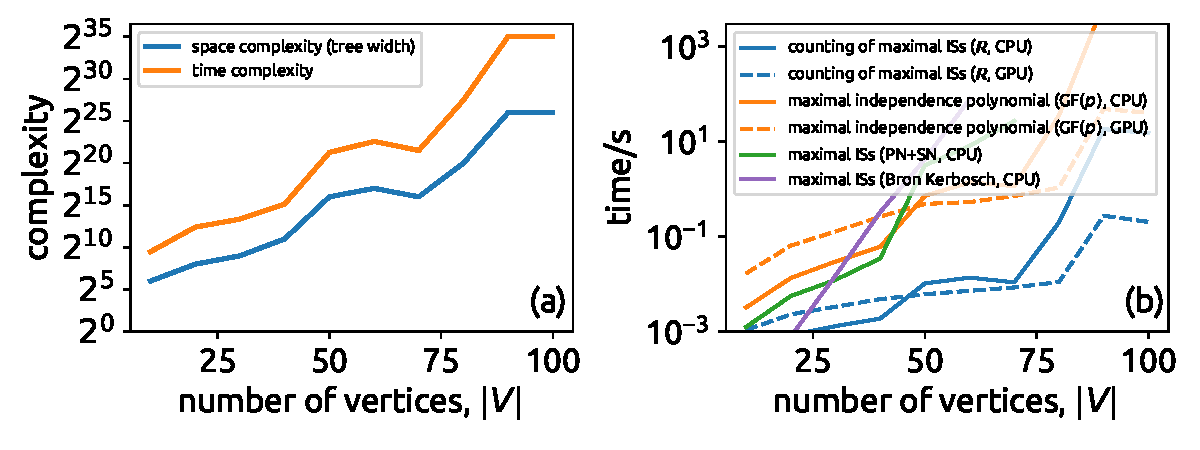
\includegraphics[width=\textwidth, trim={0cm 0cm 0cm 0cm}, clip]{figures/fig2.pdf}
    \caption{Benchmark results for computing different properties of maximal independent sets on a random three regular graph with different tensor element types.
    (a) treewidth versus the number of vertices for the benchmarked graphs. 
    (b) The computing time for calculating the number of independent sets and enumerate all MISs.
    }
    \label{fig:benchmark-maximal}
\end{figure}


\subsection{Matching problem}
A $k$-matching in a graph $G=(V,E)$ is a set of $k$ edges, no two of which have a vertex in common.
We map an edge $(u, v) \in E$ to a degree of freedom $\langle u, v\rangle \in \{0, 1\}$ in a tensor network,
where $1$ means this edge is in the set and $0$ otherwise.
To characterize the matching, one can define a tensor of rank $d(v) = |N(v)|$ on vertex $v$
\begin{equation}
    W_{\langle v, n_1\rangle, \langle v, n_2 \rangle, \ldots, \langle v, n_{d(v)}\rangle} = \begin{cases}
        1, & \sum_{i=1}^{d(v)} \langle v, n_i \rangle \leq 1,\\
        0, & \text{otherwise},
    \end{cases}
\end{equation}
and a tensor of rank $1$ on the bond
\begin{equation}
    B(w_{\langle u,v \rangle})_{\langle u, v\rangle} = \begin{cases}
    1, & \langle u, v \rangle = 0 \\
    x^{w_{\langle u,v \rangle}}_{\langle u, v\rangle}, & \langle u, v \rangle = 1,
\end{cases}
\end{equation}
where label $\langle v, u \rangle$ is equivalent to $\langle u,v\rangle$.
The vertex tensor specifies the constraint that a vertex cannot be shared by two edges in the matched set,
while an edge tensor carries the weights as the target to optimize.
Let $x_{\langle u,v\rangle}^{w_{\langle u,v\rangle}}=x$, the tensor network contraction gives us the matching polynomial
\begin{equation}
    M(G, x) = \sum\limits_{k=1}^{|V|/2} c_k x^k,
\end{equation}
where $k$ is the size of a matched edges set, and a coefficients $c_k$ is the number of $k$-matchings.

\subsection{Vertex coloring}
Let $G=(V,E)$ be a graph, a vertex coloring is an assignment of colors to each vertex $v\in V$ such that no edge connects two identically colored vertices. 
In a $k$-coloring problem, the number of different colors can be used is limited to less or equal to $k$.
Let us use the 3-coloring problem as an example to show how to characterize with local tensors.
For each vertex $v \in V$, we associate a degree of freedom $c_v\in\{0,1,2\}$ to it.
Then we define a vertex tensor labelled by it as
\begin{equation}
    W(v) = \left(\begin{matrix}
        r_v\\
        g_v\\
        b_v
    \end{matrix}\right),
\end{equation}
where $r_v$, $g_v$ and $b_v$ are colors for labeling the configurations.
For each edge $(u, v)$, we specify the constraint carrying a weight $w_{uv}$ on it by defining an edge tensor labelled by $(c_u, c_v)$ as
\begin{equation}
    B(x, w_{uv}) = \left(\begin{matrix}
        0 & x^{w_{uv}} & x^{w_{uv}}\\
        x^{w_{uv}} & 0 & x^{w_{uv}}\\
        x^{w_{uv}} & x^{w_{uv}} & 0
    \end{matrix}\right).
\end{equation}
The number of possible colorings can be obtained by contracting this tensor network by setting $r_v, g_v$ and $b_v$ to $1$.
Let $x^{w_{uv}} = x$, we have a graph polynomial,
in which the $k$-th coefficient is the number of coloring with $k$ bonds satisfied.
If a graph is colorable, the maximum order of this polynomial should be equal to the number of edges in this graph.
Similarly, one can define the $k$-coloring problem on edges by defining the tensor network on the line graph of $G$.

\subsection{Cutting problem}
In graph theory, a cut is a partition of the vertices of a graph into two disjoint subsets,
which is also known as the boolean spin glass problem in statistic physics.
Let $G=(V,E)$ be a graph, to reduce the cutting problem on $G$ to the contraction of a tensor network, we first define a boolean degree of freedom $s_v\in\{0, 1\}$ for each vertex $v\in V$.
Then for each edge $(u,v)\in E$, we define an edge matrix labelled by $s_us_v$ as
\begin{equation}
    B(x, w_{uv}) = \left(\begin{matrix}
        1 & x_{v}^{w_{uv}}\\
        x_{u}^{w_{uv}} & 1
    \end{matrix}\right),
\end{equation}
where variables $x_u$ and $x_v$ represents a cut on this edge or a domain wall in an spin glass.
Let $x_u^{w_{uv}} = x_v^{w_{uv}} = x$, we have a graph polynomial similar to previous ones,
where its $k$th coefficient is two times the number of cuts with size $k$ (i.e. cutting $k$ edges).

\subsection{Dominating Set}
In graph theory, a dominating set for a graph $G = (V, E)$ is a subset $D \subseteq V$ such that every vertex not in $D$ is adjacent to at least one member of $D$.
To reduce this problem to the contraction of a tensor network, we first map a vertex $v\in V$ to a boolean degree of freedom $s_v\in\{0, 1\}$.
Then for each vertex $v\in V$ we define a tensor on its closed neighborhood $\{v\} \cup N(v)$ as
\begin{equation}
T(x, w_v)_{s_1,s_2,\ldots,s_{|N(v)|},s_v} = \begin{cases}
    0_v & s_1=s_2=\ldots=s_{|N(v)|}=s_v=0,\\
    1_v & s_v=0,\\
    x^{w_v} & \text{otherwise},
\end{cases}
\end{equation}
where $w_v$ is the weight of vertex $v$.
This tensor means if both $v$ and its neighbouring vertices are not in $D$, i.e., $s_1=s_2=\ldots=s_{|N(v)|}=s_v=0$,
this configuration is forbidden because $v$ is not adjacent to any member in the set.
Otherwise, if $v$ is in $D$, this tensor contributes a multiplicative factor $x_v^{w_v}$ to the output.
The graph polynomial for the dominating set problem is known as the domination polynomial~\cite{Alikhani2009},
which is defined as
\begin{equation}
D(G, x) = \sum_{k=0}^{\gamma(G)} d_k x^k,
\end{equation}
where $d_k$ is the number of dominating sets of size $k$.

\subsection{Boolean satisfiability Problem}
The boolean satisfiability problem is the problem of determining if there exists an interpretation that satisfies a given boolean formula.
One can specify a satisfiable problem in the conjuctive normal form (CNF): a conjuction of disjunctions of boolean literals,
where a disjunction of boolean literals is also named a clause.
To reduce the problem of solving CNF to a tensor network contraction, we first map a boolean literal $a$ and its negation $\neg a$ to a same degree of freedom (label) $s_a \in \{0, 1\}$,
where 0 stands for variable $a$ having value \texttt{false} while 1 stands for having value \texttt{true}.
Then we map a clause to a tensor. For example, the $k$-th clause $\neg a \vee b \vee \neg c$ can be mapped to a tensor labeled by $(s_a, s_b, s_c)$.
\begin{equation}
C_{k} = \left(\begin{matrix}
\left(\begin{matrix}
x^{w_k} & x_{b}^{w_k} \\
x_a^{w_k} & x_{ab}^{w_k}
\end{matrix}\right) \\
\left(\begin{matrix}
x_{c}^{w_k} & x_{bc}^{w_k} \\
1_{ac} & x_{abc}^{w_k}
\end{matrix}\right)
\end{matrix}\right),
\end{equation}
where a weight $w_k$ is associated with a clause. There is only one entry $(s_a, s_b, s_c) = (1, 0, 1)$ that makes this clause unsatisfied.
If we contract this tensor network, we will get a multiplicative factor $x$ whenever there is a clause satisfied.
Let $x^{w_k}_{\ldots} = x$, one can get a polynomial, in which the $k$-th coefficient gives the number of assignments with $k$ clauses satisfied.

\subsection{Set packing}
Set packing is the hypergraph generalization of the maximum independent set problem, where a set corresponds to a vertex and an element corresponds to a hyperedge.
To solve the set packing problem, we can just remove the rank-2 restriction of the edge tensor in \Eq{eq:edgetensor}
\begin{equation}
    B_{s_u,s_v,\ldots, s_w} = \begin{cases}
        1, & s_u+s_v+\ldots+s_w\leq 1,\\
        0, & \text{otherwise}.
    \end{cases}
\end{equation}

\section{Bounding the MIS enumeration space}\label{sec:bounding}
\begin{figure}
    \centering
    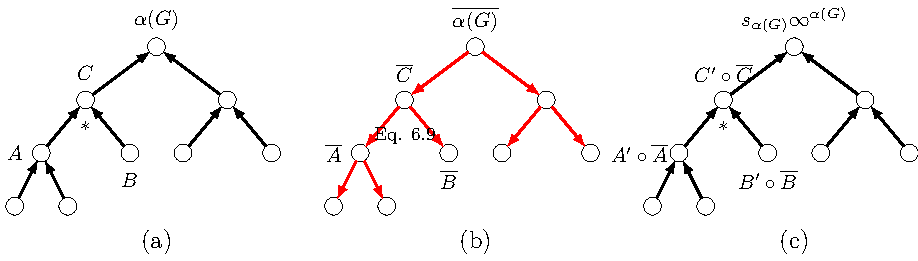
\includegraphics[width=0.9\textwidth, trim={0cm 0cm 0cm 0cm}, clip]{figures/masktree.pdf}
    \caption{Bounded enumeration of maximum independent sets. In these graphs, a circle is a tensor, an arrow specifies execution direction of a function and $\circ$ is the Hadamard (element-wise) multiplication. $\overline A$ means the boolean mask of $A$. (a) is the forward pass with algebra \Eq{eq:tropical} for computing $\alpha(G)$.
     (b) is the backward pass for computing boolean gradients as masks.
     (c) is the masked forward pass with algebra \Eq{eq:countingtropicalset} for enumerating configurations.}
     \label{fig:bounding}
\end{figure}

When we use the algebra in \Eq{eq:countingtropicalset} to enumerate all MIS configurations, we find that the program stores significantly more intermediate configurations than necessary and thus incur significant overheads in space.
To speed up the computation and reduce space overhead, we bound the searching space using the information from the computation of the MIS size $\alpha(G)$.
As shown in \Fig{fig:bounding}, (a) we first compute the value of $\alpha(G)$ with tropical algebra and cache all intermediate tensors.
(b) Then, we compute a boolean mask for each cached tensor, where we use a boolean true to represent a tensor element having a contribution to the MIS (i.e.\ with a non-zero gradient) and boolean false otherwise.
(c) Finally, we perform masked tensor network contraction (i.e.\ discarding the unnecessary intermediate configurations) using the element type with the algebra in \Eq{eq:countingtropicalset} to obtain all MIS configurations.
Note that these masks in fact correspond to tensor elements with non-zero gradients with respect to the MIS size; we compute these masks by back propagating the gradients.
To derive the back-propagation rule for tropical tensor contraction,
we first reduce the problem to finding the back-propagation rule of a tropical matrix multiplication $C = A B$.
Since $ C_{ik} = \bigoplus_{j} \ A_{ij} \odot B_{jk} = \max_{j} \ A_{ij} \odot B_{jk}$ with tropical algebra, we have the following inequality
\begin{equation}
    A_{ij} \odot B_{jk} \leq C_{ik}.
\end{equation}
Here $\leq$ on tropical numbers are the same as the real-number algebra.
The equality holds for some $j'$, which means $A_{ij'}$ and $B_{j'k}$ have contributions to $C_{ik}$.
Intuitively, one can use this relation to identify elements with nonzero gradients in $A$ and $B$,
but if doing this directly, one loses the advantage of using BLAS libraries~\cite{TropicalGEMM} for high performance.
Since $A_{ij} \odot B_{jk} = A_{ij} + B_{jk}$, one can move $B_{jk}$ to the right hand side of the inequality: 
\begin{equation}
    A_{ij} \leq C_{ik} \odot B_{jk}^{\circ -1}
\end{equation}
where ${}^{\circ -1}$ is the element-wise multiplicative inverse on tropical algebra (which is the additive inverse on real numbers).
The inequality still holds if we take the minimum over $k$: 
\begin{equation}
    A_{ij} \leq \min_{k}(C_{ik} \odot B_{jk}^{\circ -1}) = \left(\max_{k} \left(C_{ik}^{\circ -1} \odot B_{jk} \right) \right)^{\circ -1} = \left(\bigoplus_{k} \left(C_{ik}^{\circ -1} \odot B_{jk} \right) \right)^{\circ -1} = \left( C^{\circ-1} B^{\mathsf{T}} \right)^{\circ -1}_{ij}.
\end{equation}
On the right hand side, we transform the operation into a tropical matrix multiplication so that we can utilize the fast tropical BLAS routines~\cite{TropicalGEMM}.
Again, the equality holds if and only if the element $A_{ij}$ has a contribution to $C$ (i.e.\ having a non-zero gradient).
Let the gradient mask for $C$ be $\overline C$; the back-propagation rule for gradient masks reads
\begin{equation}\label{eq:adrule}
\overline{A}_{ij} = \delta \left(A_{ij}, \left( \left( C^{\circ-1} \circ \overline C \right) B^{\mathsf{T}} \right)_{ij}^{\circ -1} \right),
\end{equation}
where $\delta$ is the Dirac delta function that returns one if two arguments have the same value and zero otherwise, $\circ$ is the element-wise product, boolean false is treated as the tropical number $\mymathbb{0}$, and boolean true is treated as the tropical number $\mymathbb{1}$.
This rule defined on matrix multiplication can be easily generalized to tensor contraction by replacing the matrix multiplication between $C^{\circ-1} \circ \overline C$ and $B^{\mathsf{T}}$ by a tensor contraction.
With the above method, one can significantly reduce the space needed to store the intermediate configurations by setting the tensor elements masked false to zero during contraction.

\section{The fitting approach to computing the independence polynomial}\label{sec:finitefield}
In this section, we propose to find the independence polynomial by fitting $\alpha(G)+1$ random pairs of $x_{i}$ and $y_{i} = I(G,x_{i})$. One can then compute the independence polynomial coefficients $a_{i}$ by solving the linear equation: 
\begin{equation}
\left(\begin{matrix}
1 & x_0 & x_0^2 & \ldots & x_0^{\alpha(G)} \\
1 & x_1 & x_1^2 & \ldots & x_1^{\alpha(G)} \\
\vdots & \vdots & \vdots &\ddots & \vdots \\
1 & x_{\alpha(G)} & x_{\alpha(G)}^2 & \ldots & x_{\alpha(G)}^{\alpha(G)}
\end{matrix}\right)
\left(\begin{matrix}
a_0 \\ a_1 \\ \vdots \\ a_{\alpha(G)}
\end{matrix}\right)
= \left(\begin{matrix}
y_0 \\ y_1 \\ \vdots \\ y_{\alpha(G)}
\end{matrix}\right).\label{eq:lineareq}
\end{equation}
With this approach, we do not incur the linear overhead in space. However, because the independence polynomial coefficients can have a huge order-of-magnitude range, if we use floating point numbers in the computation, the round-off errors can be significant for the counting of large-size independent sets.
In addition, the number could easily overflow if we use fixed-width integer types.
The big integer type is also not a good option because big integers with varying width can be very slow and is incompatible with GPU devices. These problems can be solved by introducing a finite-field algebra $\text{GF}(p)$:
\begin{equation}
\eqname{GF$(p)$}
\begin{split}
    x ~\oplus~ y &= x+y\pmod p,\\
    x ~\odot~ y &= xy\pmod p,\\
    \mymathbb{0} &= 0,\\
    \mymathbb{1} &= 1.
\end{split}\label{eq:finitefield}
\end{equation}
With a finite-field algebra, we have the following observations:
\begin{enumerate}
    \item One can use Gaussian elimination~\cite{Golub2013} to solve the linear equation \Eq{eq:lineareq} since it is a generic algorithm that works for any elements with field algebra. The multiplicative inverse of a finite-field algebra can be computed with the extended Euclidean algorithm.
    \item Given the remainders of a larger unknown integer $x$ over a set of co-prime integers $\{p_1, p_2, \ldots, p_n\}$,
    $x \pmod {p_1 \times p_2 \times \ldots \times p_n}$ can be computed using the Chinese remainder theorem. With this, one can infer big integers from small integers.
\end{enumerate}
With these observations, we develop Algorithm~\ref{alg:finitefield} to compute the independence polynomial exactly without introducing space overheads.
The algorithm iterates over a sequence of large prime numbers until convergence.
In each iteration, we choose a large prime number $p$, and contract the tensor networks to evaluate the polynomial for each variable $\chi = (x_{0}, x_{1}, \ldots, x_{\alpha(G)})$ on ${\rm GF}(p)$ and denote the outputs as $(y_0, y_1, \ldots, y_{\alpha(G)}) \pmod p$.
Then we solve \Eq{eq:lineareq} using Gaussian elimination on ${\rm GF}(p)$ to find the coefficient modulo $p$, $A_p \equiv (a_0, a_1, \ldots, a_{\alpha(G)})\pmod p$.
As the last step of each iteration, we apply the Chinese remainder theorem to update $A \pmod P $ to $ A \pmod {P\times p}$, where $P$ is a product of all prime numbers chosen in previous iterations.
If this number does not change compared with the previous iteration, it indicates the convergence of the result and the program terminates.
All computations are done with integers of fixed width $W$ except the last step of applying the Chinese remainder theorem, where we use arbitrary precision integers to represent the counting.

\LinesNumberedHidden
\begin{algorithm}[!ht]
    \small
    \SetAlgoNoLine
    %\LinesNumbered
    Let $P = 1$, $W$ be the integer width, vector $\chi = (0,1,2, \ldots, \alpha(G))$, matrix $X_{ij} = (\chi_i)^j$, where $i,j = 0, 1, \ldots, \alpha(G)$\;

    \While{true}{
        compute the largest prime $p$ that $\gcd(p, P) = 1$ and $p < 2^W$\;

        \For{$i=0\ldots\alpha(G)$}{
            $y_i \pmod p$ = ${\rm contract\_tensor\_network}(\chi_i\pmod p)$ \tcp*[l]{on $\text{GF}(p)$}
        }

        $A_p = (a_0, a_1, \ldots, a_{\alpha(G)}) \pmod p = {\rm gaussian\_elimination}(X, (y_0, y_1, \ldots, y_{\alpha(G)}) \pmod p) $\;

        $A_{P\times p} = {\rm chinese\_remainder}(A_P, A_p)$\;

        \If{$A_P = A_{P \times p}$}{
            \Return $A_P$ \tcp*[l]{converged}
        }
        $P = P \times p$\;
    }\caption{Computing the independence polynomial exactly without integer overflow}\label{alg:finitefield} 
\end{algorithm}


\section{The discrete Fourier transform approach to computing the independence polynomial}\label{sec:fft}

In section~\ref{sec:indpoly}, we show that the independence polynomial can be obtained by solving the linear equation \Eq{eq:lineareq}.
Since the coefficients of the independence polynomial can range many orders of magnitude, the round-off errors in fitting can be significant if we use random floating point numbers for $x_{i}$.
In the main text, we propose to use a finite field $\text{GF}(p)$ to circumvent integer overflow and round-off errors.
One drawback of using finite field algebra is its matrix multiplication is less computational efficient compared with floating point matrix multiplication.
Here, we give an alternative method based on discrete Fourier transform with controllable round off errors.
Instead of choosing $x_{i}$ as random numbers, we can choose them such that they form a geometric sequence in the complex domain $x_j = r\omega^j$, where $r \in \mathbb{R}$ and $\omega = e^{-2\pi i/( \alpha(G)+1)}$. The linear equation thus becomes
\begin{equation}
\left(\begin{matrix}
1 & r & r^2 & \ldots & r^{\alpha(G)} \\
1 & r\omega & r^2\omega^2 & \ldots & r^{\alpha(G)} \omega^{\alpha(G)} \\
\vdots & \vdots & \vdots &\ddots & \vdots \\
1 & r\omega^{\alpha(G)} & r^2\omega^{2{\alpha(G)}} & \ldots & r^{\alpha(G)}\omega^{{\alpha(G)}^2}
\end{matrix}\right)
\left(\begin{matrix}
a_0 \\ a_1 \\ \vdots \\ a_{\alpha(G)}
\end{matrix}\right)
= \left(\begin{matrix}
y_0 \\ y_1 \\ \vdots \\ y_{\alpha(G)}
\end{matrix}\right).
\end{equation}

Let us rearrange the coefficients $r^j$ to $a_j$, the matrix on the left side becomes the discrete Fourier transform matrix. Thus, we can obtain the coefficients by inverse Fourier transform $\vec a_r = {\rm FFT^{-1}}(\omega) \cdot \vec y$, where $(\vec a_r)_j = a_j r ^j$.
By choosing different $r$, one can obtain better precision in low independent set size region by choosing $r<1$ or high independent set size region by choosing $r>1$.

\section{Integer sequence formed by the number of independent sets}

We computed the number of independent sets on square lattices and King's graphs
with our generic tensor network contraction algorithm on GPUs.
The tensor element type is finite-field algebra so that we can reach arbitrary precision.
We also computed the independence polynomial exactly for these lattices which can be found in our \href{https://github.com/GiggleLiu/NoteOnTropicalMIS/tree/master/data}{Github repo}.


\begin{table}[h]
\caption{The number of independent sets for square lattice graphs of size $L\times L$. This forms the integer sequence \href{https://oeis.org/A006506}{OEIS A006506}.
Here we only include two updated entries for $L=38,39$, which, to our knowledge, has not been computed before~\cite{Butera2014}.
}
\begin{center}
\scalebox{0.9}{
\begin{tabular}{|c| >{\centering\arraybackslash} p{0.95\linewidth}|}
 \hline $L$  & square lattice graphs \\
 \hline $38$ & 616 412 251 028 728 207 385 738 562 656 236 093 713 609 747 387 533 907 560 081 990 229 746 115 948 572 583 817 557 035 128 726 922 565 913 748 716 778 414 190 432 479 964 245 067 083 441 583 742 870 993 696 157 129 887 194 203 643 048 435 362 875 885 498 554 979 326 352 127 528 330 481 118 313 702 375 541 902 300 956 879 563 063 343 972 979\\
 \hline $39$ &  29 855 612 447 544 274 159 031 389 813 027 239 335 497 014 990 491 494 036 487 199 167 155 042 005 286 230 480 609 472 592 158 583 920 411 213 748 368 073 011 775 053 878 033 685 239 323 444 700 725 664 632 236 525 923 258 394 737 964 155 747 730 125 966 370 906 864 022 395 459 136 352 378 231 301 643 917 282 836 792 261 715 266 731 741 625 623 207 330 411 607\\
  \hline
\end{tabular}
}
\end{center}
\label{tbl:squaregrid}
\end{table}
% online digit seperator: https://www.browserling.com/tools/thousands-separator

\section{Computing maximum sum combination}\label{sec:maxsum}
Given two sets $A$ and $B$ of the same size $n$.
It is known that the maximum $n$ sum combination of $A$ and $B$ can be computed in time $n\log(n)$.
The standard approach to solve the sum combination problem requires storing the variables in a heap - a highly dynamic binary tree structure which can can be much slower to manipulate than arrays.
In the following, we show an algorithm that has roughly the same complexity (given the data range is not exponentially large)
but does not need a heap.
This algorithm first sorts both $A$ and $B$, then use the bisection to find the $n$-th largest value in the sum combination.
The key point is we can count the number of entries greater than a specific value
in the sum combination of $A$ and $B$ in linear time.
We summarize the algorithm as in Algorithm~\ref{alg:sumcombination}.

\LinesNumberedHidden
\begin{algorithm}[!ht]
    \SetKwProg{Fn}{function}{}{end}
    \small
    \SetAlgoNoLine
    Let $A$ and $B$ be two sets of size $n$\;

    \tcp{sort $A$ and $B$ in ascending order}
    $A \gets {\rm sort}(A)$\;

    $B \gets {\rm sort}(B)$\;

    \tcp{use bisection to find the $n$-th largest value in sum combination}

    ${\rm high} \gets A_n+B_n$\;

    ${\rm low} \gets A_1+B_n$\;

    \While{true}{
        ${\rm mid} \gets ({\rm high} + {\rm low}) / 2$\;

        $c \gets \texttt{count\_geq}(n, A, B, {\rm mid})$\;

        \uIf{$c > n$}{
            ${\rm low} \gets {\rm mid}$\;
        }\uElseIf{$c = n$}{
            \Return \texttt{collect\_geq}$(n, A, B, {\rm mid})$\;
        }\Else{
            ${\rm high} \gets {\rm mid}$\;
        }
    }

    \Fn{{\rm \texttt{count\_geq}}($n$, $A$, $B$, $v$)}{
        $k \gets 1$\; \tcp*[l]{number of entries in $A$ s.t. $a+b\geq v$}

        $a \gets A_{n}$\; \tcp*[l]{the smallest entry in $A$ s.t. $a+b\geq v$}

        $c \gets 0$\; \tcp*[l]{the counting of sum combinations s.t. $a+b\geq v$}

        \For{$q$ = $n, n-1 \ldots 1$}{
            $b \gets B_{n-q+1}$\;

            \While{$k < n$ \textbf{and} $a+b \geq v$}{
                $k \gets k+1$\;

                $a \gets A_{n-k+1}$\;
            }

            \uIf{$a+b \geq v$}{
                $c \gets c + k$\;
            }\Else{
                $c \gets c + k-1$\;
            }
        }
        \Return c\;
    }

    % \Fn{\rm collect\_geq($n$, $A$, $B$, $v$)}{
    %     $k \gets 1$\; \tcp*[l]{number of entries in $A$ s.t. $a+b\geq v$}

    %     $a \gets A_{n}$\; \tcp*[l]{the smallest entry in $A$ s.t. $a+b\geq v$}

    %     $S \gets \{\}$ \tcp*[l]{the sum combinations s.t. $a+b\geq v$}

    %     \For{$q$ = $n, n-1 \ldots 1$}{
    %         $b \gets B_{n-q+1}$\;

    %         \While{$k < n$ \textbf{and} $a+b \geq v$}{
    %             $k \gets k+1$\;

    %             $a \gets A_{n-k+1}$\;
    %         }

    %         \uIf{$a+b \geq v$}{
    %             $m \gets k$\;
    %         }\Else{
    %             $m \gets k-1$\;
    %         }
    %         \For{$j$ = \KwTo $1,2\ldots,m$}{
    %             $S \gets S \cup \{b + A_{n-j+1}\}$
    %         }
    %     }
    %     \Return S\;
    % }
    \caption{Fast sum combination without using heap}\label{alg:sumcombination} 
\end{algorithm}

Function \texttt{collect\_geq} is similar the \texttt{count\_geq} except the counting is replace by the item collection.
Note in function \texttt{count\_geq}, variable $k$ monotoneously increase while $q$ monotoneously decrease in each iteration,
the total number of iterations must be smaller or equal to $2n$.
Here for simplicity, we do not handle the $-\infty$s in $A$ and $B$ and the degeneracy in the sums.
They need to be taken seriously in practical implementations.

\section{Technical guide}\label{sec:technical}

This appendix covers some technical aspects of this paper, including an open source package and a gist about how to implement this package. If you are only interested in using, please checking our GitHub repository for an efficient and full featured implementation aimed for productively:
\href{https://github.com/Happy-Diode/GraphTensorNetworks.jl}{https://github.com/Happy-Diode/GraphTensorNetworks.jl}.
One can install these packages by opening a Julia REPL, type \colorbox{lightgray}{\texttt{]}} to enter the \texttt{pkg>} mode and type, e.g.
\begin{lstlisting}
pkg> add GraphTensorNetworks
\end{lstlisting}
To use it, just open Julia REPL and type

\begin{lstlisting}
julia> using GraphTensorNetworks, Graphs

julia> solve(
           IndependentSet(
               Graphs.random_regular_graph(20, 3);
               optimizer = TreeSA()
           ),
           GraphPolynomial()
       )
0-dimensional Array{Polynomial{BigInt, :x}, 0}:
Polynomial(1 + 20*x + 160*x^2 + 659*x^3 + 1500*x^4 + 1883*x^5 + 1223*x^6 + 347*x^7 + 25*x^8)
\end{lstlisting}



The first time you run the code might trigger the just in time compiling,
it will be a bit slow, but the following computing will be fast.

The code we will show below is a gist of how the above package is implemented, which is mainly for the pedagogical purpose.
It covers most of the topics in the paper without caring much about the performance.
This project depends on multiple open source packages in the Julia ecosystem:

\begin{description}
	\item[\href{https://github.com/under-Peter/OMEinsum.jl}{OMEinsum} and \href{https://github.com/Happy-Diode/OMEinsumContractionOrders.jl}{OMEinsumContractionOrders}] are packages providing the support for Einstein's (or tensor network) notation and contraction order optimizations.
    \texttt{OMEinsumContractionOrders} implements state-of-the-art algorithms for finding the optimal contraction order for a tensor network, including the KaHypar+Greedy~\cite{Gray2021, Pan2021} and local transformation based approaches~\cite{Kalachev2021},
	\item[\href{https://github.com/TensorBFS/TropicalNumbers.jl}{TropicalNumbers} and \href{https://github.com/TensorBFS/TropicalGEMM.jl}{TropicalGEMM}] are packages providing tropical number and efficient tropical matrix multiplication,
	\item[\href{https://github.com/JuliaGraphs/Graphs.jl}{Graphs}] is a package providing graph utilities, like random regular graph generator,
	\item[\href{https://github.com/JuliaMath/Polynomials.jl}{Polynomials}] is a package providing polynomial algebra and polynomial fitting,
	\item[\href{https://github.com/scheinerman/Mods.jl}{Mods} and \href{https://github.com/JuliaMath/Primes.jl}{Primes}] are packages providing finite field algebra and prime number generations.
\end{description}

They can be installed in a similar way to \texttt{GraphTensorNetworks}.
After installing the required packages, one can open a Julia REPL, then copy and paste the following code into it.

\lstinputlisting[breaklines]{../democode/demo.jl}


\end{document}
